%%%%%%%%%%%%%%%%%%%%%%%%%%%%%%%%%%%%
%                                  %
%         Thesis template           %
%                                  %
% version 1.0 04-11-13             %
%                                  %
%                                  %
%%%%%%%%%%%%%%%%%%%%%%%%%%%%%%%%%%%%


%%%%%%%%%%%%%%%%%%%%%%%%%%%%%%%%%%%%
%%
%%   Preamble
%%
%%%%%%%%%%%%%%%%%%%%%%%%%%%%%%%%%%%%

%%%%%%%%%%%%%%%%%%%%
% Document type 
%%%%%%%%%%%%%%%%%%%%

% Definition de la classe de document: article, book, report, letter, slides
% Options:  	taille de la police: 10pt, 11pt, 12pt, ...
%		format du papier: a4paper, a5paper ...
% 		stade de developpement: draft, final
%		autres: oneside, twoside, twocolumn (recto simple, recto-verso, sur deux colonne)
\documentclass[12pt, letterpaper, twoside,spanish, openright]{usach-tesis}


%%%%%%%%%%%%%%%%%%%%%%%%%
% Language and font
%%%%%%%%%%%%%%%%%%%%%%%%%

% Gestion des langues: utilisation du package babel
% Option: francais, english
% Rq: 	Dans le cas d'un document bilingue, la derniere langue indiquée est la langue dominante  
%	pour changer de langue: \selectlanguage{english}

%\usepackage[francais]{babel}
\usepackage[spanish,es-uppernames,es-tabla]{babel}
%\usepackage[francais,english]{babel}
%\usepackage[english,francais]{babel}

% Definition de macro pour changer de langue
%\newcommand{\en}{\selectlanguage{english}}
%\newcommand{\fr}{\selectlanguage{francais}}


% Using of vectorial fonts
\usepackage{lmodern}
% \usepackage{aeguill} % using adobe font

% Accents managning
\usepackage[T1]{fontenc} % using Latex font with accents
\usepackage[utf8]{inputenc} % emphasised character are recognized (or \usepackage[latin1]{inputenc} for os which did not use UTF-8)


%%%%%%%%%%%%%%%%
% Page setting
%%%%%%%%%%%%%%%%

% Margin definition  (by default write 66 characters per line, for an optimal readability !!!!)
% Option: 	a4paper
%		textwidth, textheight
%		top, bottom, left, right
\usepackage[top=2cm, bottom=2cm, left=3cm, right=2cm, letterpaper,includehead]{geometry}
%\usepackage[top=2cm, bottom=2cm, left=3cm, right=2cm, letterpaper]{geometry}

% Style de page: 	empty : le header et le footer sont vide
%			plain : le header est vide et le footer contient le numero de page
%			headings : le header contient le numero de page et un titre
% Changement de style: \thispagestyle{style} et \pagestyle{style}
%\pagestyle{headings}


% Sub figure using
\usepackage{subfigure}

% Positioning in flotting  (for tables and figures)
\usepackage{float}

%%%%%%%%%%%%%%%%%%%%%%%%%%%%%%%%%%%%%%%%%%
% Table of contents configuration 
%%%%%%%%%%%%%%%%%%%%%%%%%%%%%%%%%%%%%%%%%%

% Inclusion dans la table des matieres, de la liste des figures, des tables, de la bibliographie ...
% Options : 	nottoc: desactive l'inclusion de la table de matiere
% 		notlof: desactive l'inclusion de la liste des tables
%		notlot: desactive l'inclusion de la liste des figures
%		notbib: desactive l'inclusion de la bibliographie
%		notindex: desactive l'inclusion de l'index
%\usepackage[nottoc]{tocbibind}

%%%%%%%%%%%%%%%%%%%%%
% Link using
%%%%%%%%%%%%%%%%%%%%%
\usepackage[%
    bookmarks         = true,%     % Signets
    bookmarksnumbered = true,%     % Signets numérotés%
    bookmarksopen     = true,%	   % Signets ouverts
    colorlinks        = true,%     % Liens en couleur : true ou false
    urlcolor          = blue,%     % Couleur des liens externes
    linkcolor         = black,
    citecolor         = black,
    filecolor         = black]{hyperref}%                   % Utilisation de HyperTeX

\usepackage{url}	% for internet link

%%%%%%%%%%%%%%%%%%
% Other packages
%%%%%%%%%%%%%%%%%%
%\usepackage{showframe}
% Include images
\usepackage{graphicx}
\usepackage{etex}
\usepackage{tikz,pgfplots}
%\usepackage{pgfplots}

% Specifies the directory where pictures are stored
\graphicspath{{img/}} 

% Use the "Natbib" style for the references in the Bibliography
\usepackage[square, numbers, comma, sort&compress]{natbib}  

% Formate code: C/C++ ,Java ...
\usepackage{listings}

% Write algorithms
\usepackage{algorithm,algorithmic}


% For symbole like degree
\usepackage{gensymb}

% Math AMS : enables an advance seeting of the equation, to number it ...
\usepackage{amsfonts}
\usepackage{amssymb}
\usepackage{amstext}
\usepackage{amsmath}

% Draw figure
\usepackage{pstricks}
\usepackage{pstricks-add}
\usepackage{pst-text}
\usepackage{pstcol,multido}
\usepackage{pst-3dplot}

% enable doublespacing
\usepackage{setspace}
%\doublespacing
\onehalfspacing
\usepackage{indentfirst}
\usepackage{times}
%\usepackage{pslatex} %Times font

% Draw tables.
\usepackage{multirow} 

\usepackage[toc]{glossaries}
%\usepackage[authordate]{biblatex-chicago}
%\usepackage[longnamesfirst,nonamebreak]{natbib}
%\usepackage{natbib}


% Change "Capitulo" to uppercase
\makeatletter
\renewcommand{\spanishchaptername}{CAP\'ITULO}
\makeatother


%% ----------------------------------------------------------------
% Header and footer with the fancyhdr package
\usepackage{fancyhdr}
\pagestyle{fancy}

%\setstretch{1.3}  % It is better to have smaller font and larger line spacing than the other way round

% Define the page headers using the FancyHdr package and set up for one-sided printing
%\fancyhead{}  % Clears all page headers and footers
%\rhead{\thepage}  % Sets the right side header to show the page number
%\lhead{}  % Clears the left side page header

\DeclareMathOperator*{\median}{median}

%\pagestyle{fancy}  % Finally, use the "fancy" page style to implement the FancyHdr headers

%% ----------------------------------------------------------------


%%%%%%%%%%%%%%%%%%%%%%%%%%%%%%%%%%%%
%%
%%   Document
%%
%%%%%%%%%%%%%%%%%%%%%%%%%%%%%%%%%%%%
\begin{document}
%There's a workaround to get table of contents to be clickable so I can navigate through chapters a bit easier as I'm writing.
 \pdfstringdefDisableCommands{%
   \let\MakeUppercase\relax
} 

\definecolor{forestgreen}{rgb}{0.13,0.54,0.13}


%% ----------------------------------------------------------------

%  First pages (Cubierta, Caratula)
\newgeometry{top=3cm, bottom=3cm, left=3cm, right=3cm,letterpaper,ignoreall}
\begin{titlepage}
\begin{center}
\textsc{UNIVERSIDAD DE SANTIAGO DE CHILE}\\ 
\textsc{FACULTAD DE INGENIERÍA}\\ 
\null % Empty line
%\vfill
\null
\null
%\vfill


\vspace*{\fill}
\textsc{Evaluación de métodos de detección de siluetas para clasificación de acciones basado en MuHAVI un conjunto de datos para reconocimiento de acciones humanas}\\[0.5cm]
\vspace*{\fill}
\vfill
\textsc{Jorge Antonio Sepúlveda Ortega}\\ % Your name
%{\large \today}\\[3cm] % Date, change the \today to a set date if you want to be precise
{\large \today}  % Date, change the \today to a set date if you want to be precise
%\vfill % Fill the rest of the page with whitespace
\end{center}
\end{titlepage}
\newpage\thispagestyle{empty}\mbox{}

\begin{titlepage}
\begin{center}
\textsc{UNIVERSIDAD DE SANTIAGO DE CHILE}\\ 
\textsc{FACULTAD DE INGENIERÍA}\\ 
\null % Empty line
%\vfill

\null
\null
\vfill


\vspace*{\fill}
\textsc{Evaluación de métodos de detección de siluetas para clasificación de acciones basado en MuHAVI un conjunto de datos para reconocimiento de acciones humanas}\\[0.5cm]
Trabajo de Titulación presentado en conformidad a los requisitos  para obtener el Título de Ingeniero Civil en Informática
\vspace*{\fill}

\begin{minipage}[c]{0.5 \textwidth}
\begin{flushright}
\emph{Profesor guía:} \textsc{Sergio Velastín}
\end{flushright}
\end{minipage}


\vfill
\textsc{Jorge Antonio Sepúlveda Ortega}\\ % Your name
{\large \today} % Date, change the \today to a set date if you want to be precise
%\vfill % Fill the rest of the page with whitespace
\end{center}
\end{titlepage}

\newpage\thispagestyle{empty}\mbox{}
\restoregeometry


%% ----------------------------------------------------------------
% Begin Roman style (i, ii, iii, iv...) page numbering
\frontmatter

%\setstretch{1.3}  % Reset the line-spacing to 1.3 for body text (if it has changed)
% The Acknowledgements page, for thanking everyone
\agradecimientos{
\addtocontents{toc}{\vspace{1em}}  % Add a gap in the Contents, for aesthetics
Gracias totales\ldots
%\agradecimientos{
\addtocontents{toc}{\vspace{1em}}  % Add a gap in the Contents, for aesthetics

Quisiera agradecer en primer lugar a mi familia, especialmente a mi esposa por su comprensión, apoyo durante este camino. A mis hijos por la paciencia. Mencionar a mi hija del ``medio'' por su ayuda en la correción ortográfica y la redacción de los primeros capítulos. \\

Agradecer también a mi profesor guía, Dr. Sergio A. Velastín por su disposición de aceptarme en primer lugar como su alumno tesista sin conocerme previamente. Por los consejos, opiniones, puntos de vistas que espero esten bien reflejados en este trabajo. También, por las amenas charlas que surgían en las reuniones de avances, más alla del trabajo de tesis. \\

Me gustaría mencionar en estos agradecimientos a los académicos del departamento de Ingeniería Informática. Por la dedicación y motivación del trabajo en clases. Sería injusto mencionar sólo algunos, y dejar a otros fuera. También agradecer a don Miguel Fuentes, coordinador del programa vespertino, lo más probable que él no recuerde, pero fue él la primera persona que me aconsejó para entrar al programa vespertino.\\

Muchas Gracias.\\

}
}
\clearpage  % End of the Acknowledgements
%% ----------------------------------------------------------------

% The "Funny Quote Page"
\pagestyle{empty}  % No headers or footers for the following pages

\null\vfill
% Now comes the "Funny Quote", written in italics
\textit{``Whenever you find yourself on the side of the majority, it is time to pause and reflect.''}

\begin{flushright}
Mark Twain
\end{flushright}

\vfill\vfill\vfill\vfill\vfill\vfill\null
\clearpage  % Funny Quote page ended, start a new page
%% ----------------------------------------------------------------
% The Abstract Page
%\setstretch{1.3}  % Reset the line-spacing to 1.3 for body text (if it has changed)
\resumen{
\addtocontents{toc}{\vspace{1em}}  % Add a gap in the Contents, for aesthetics

The Thesis Abstract is written here (and usually kept to just this page). The page is kept centered vertically so can expand into the blank space above the title too\ldots


}
\pagestyle{empty}
\clearpage  % Abstract ended, start a new page

%% ----------------------------------------------------------------

\pagestyle{empty}  %The page style headers have been "empty" all this time, now use the "fancy" headers as defined before to bring them back


%% ----------------------------------------------------------------
\tableofcontents  % Write out the Table of Contents

%% ----------------------------------------------------------------
\listoffigures  % Write out the List of Figures

%% ----------------------------------------------------------------
\listoftables  % Write out the List of Tables




%% ----------------------------------------------------------------
\fancyfoot{} % clear all fields
\fancyhead[RO,LE]{\slshape \leftmark}
\fancyhead[LO,RE]{\thepage}
\mainmatter	  % Begin normal, numeric (1,2,3...) page numbering
\pagestyle{fancy}  % Return the page headers back to the "fancy" style


\chapter{Introducción}\label{chap:capitulo_1}
\section{Antecedentes y motivación}
\indent Visión por computador es una disciplina que intenta emular las capacidades de la visión humana para identificar y clasificar diferentes objetos desde una imagen. Es un área de investigación muy amplia, que se entrelaza con diferentes campos de investigación en el ámbito de las ciencias de la computación y el desarrollo tecnológico. Tiene como desafío facilitar máquinas computacionales con capacidad de percepción humana, en otras palabras comprender el medio ambiente, tomar acciones, aprendizaje, y mejorar desempeño de acciones tomadas. Visión por computador intenta hacer una descripción del mundo que los seres humanos pueden observar, a través de imágenes para hacer una reconstrucción de sus principales propiedades.

\indent Hay en el último tiempo un constante desarrollo de nuevas técnicas y aparatos tecnológicos (figura \ref{fig:aplicaciones_vision_por_computador}), que incorporan algoritmos empleados en visión por computador, en heterogéneos campos de aplicación. Se está experimentando algoritmos inteligentes en vehículos que permiten evitar obstáculos, reconocer peatones o viajar de un punto a otro sin la intervención de un conductor. En dispositivos audiovisuales, como cámaras fotográficas digitales, algoritmos de reconocimiento de figuras y rostros es una característica normal incluida en estos artefactos. Se utilizan además, las técnicas de análisis y reconocimiento de patrones en imágenes médicas, o clasificación de acciones humanas en cámaras de vigilancia, entre muchas otras aplicaciones.


\begin{figure}
\centering     %%% not \center
\subfigure[Evitar obstáculos]{\label{fig:Figure_A}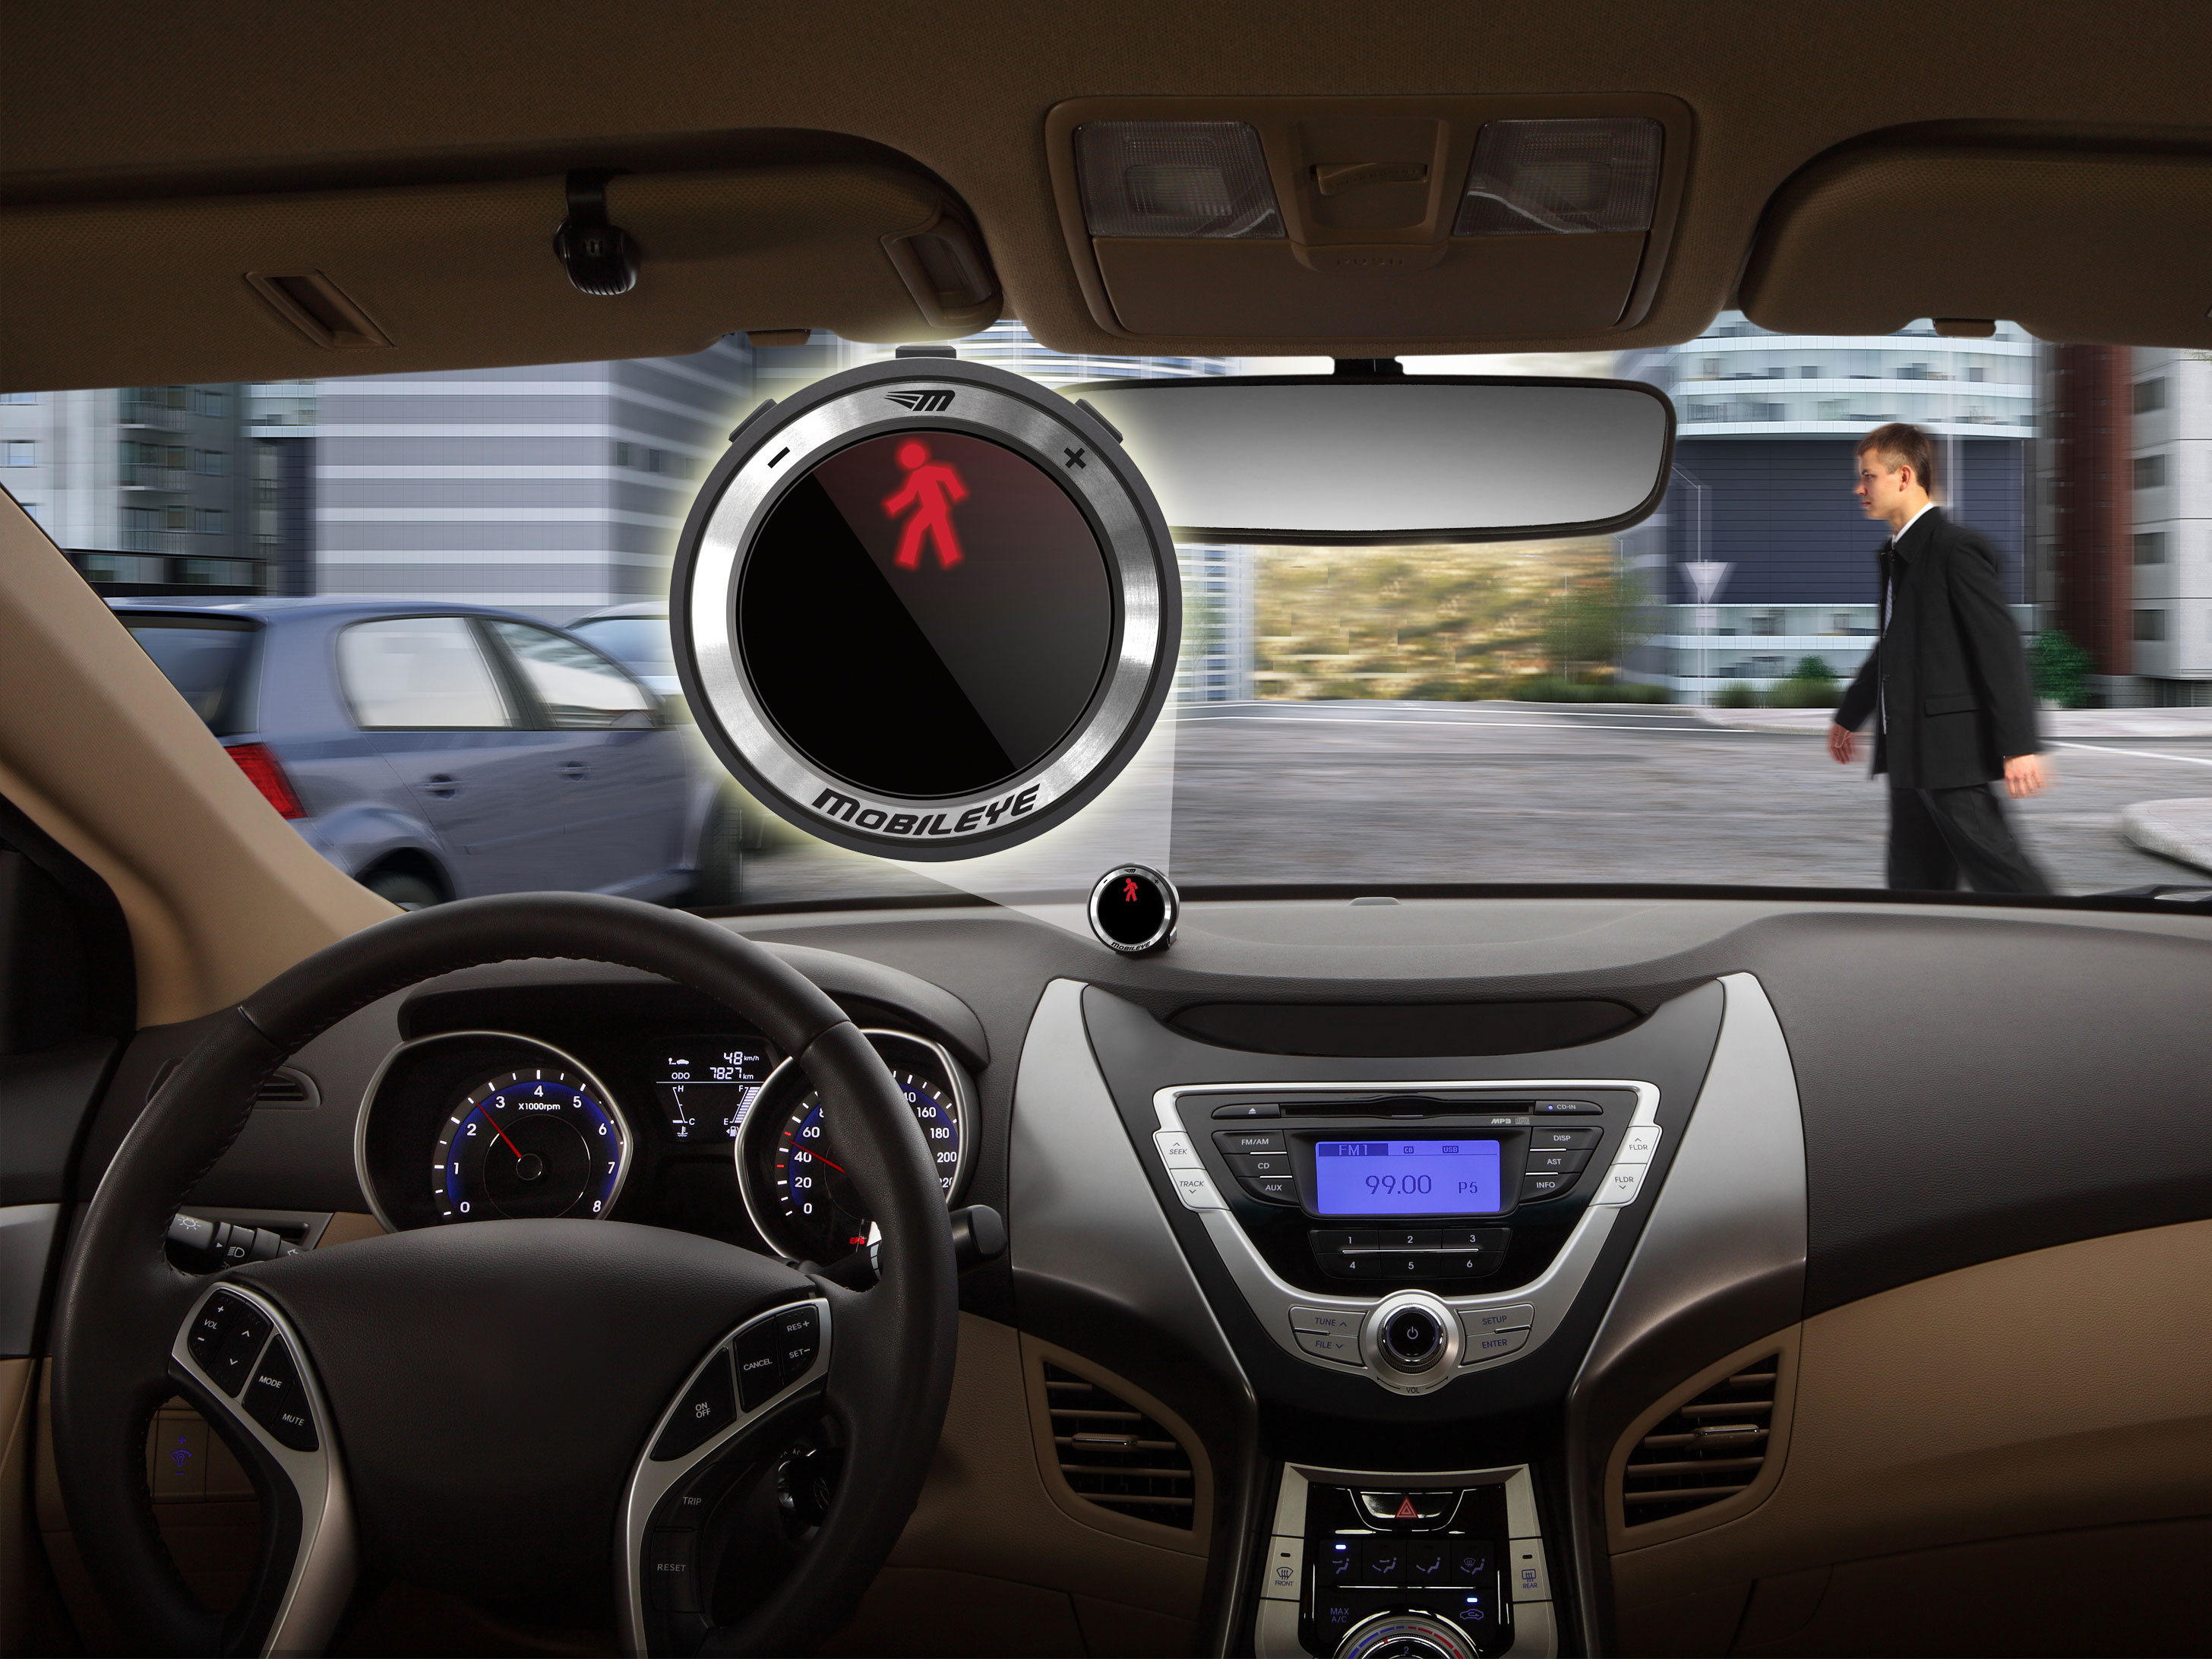
\includegraphics[width=50mm]{img/ch1/MobileEyemaster}}
\subfigure[Reconocimiento de vehículos]{\label{fig:Figure_B}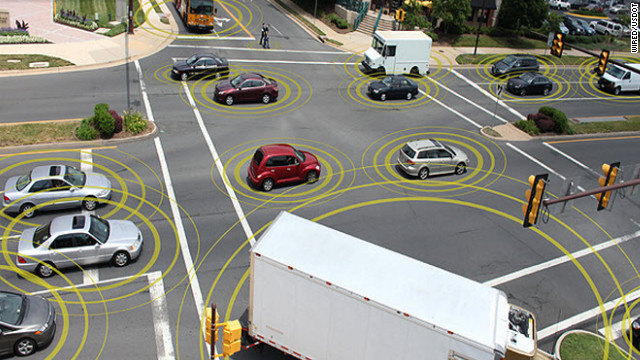
\includegraphics[width=50mm]{img/ch1/self-driving-cars}}
\subfigure[Reconocimiento de peatones]{\label{fig:Figure_C}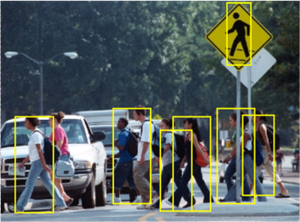
\includegraphics[width=50mm]{img/ch1/crossing}}
\subfigure[Experimentación con vehículos autónomos \tiny{(Figure courtesy Google \copyright )}]{\label{fig:Figure_D}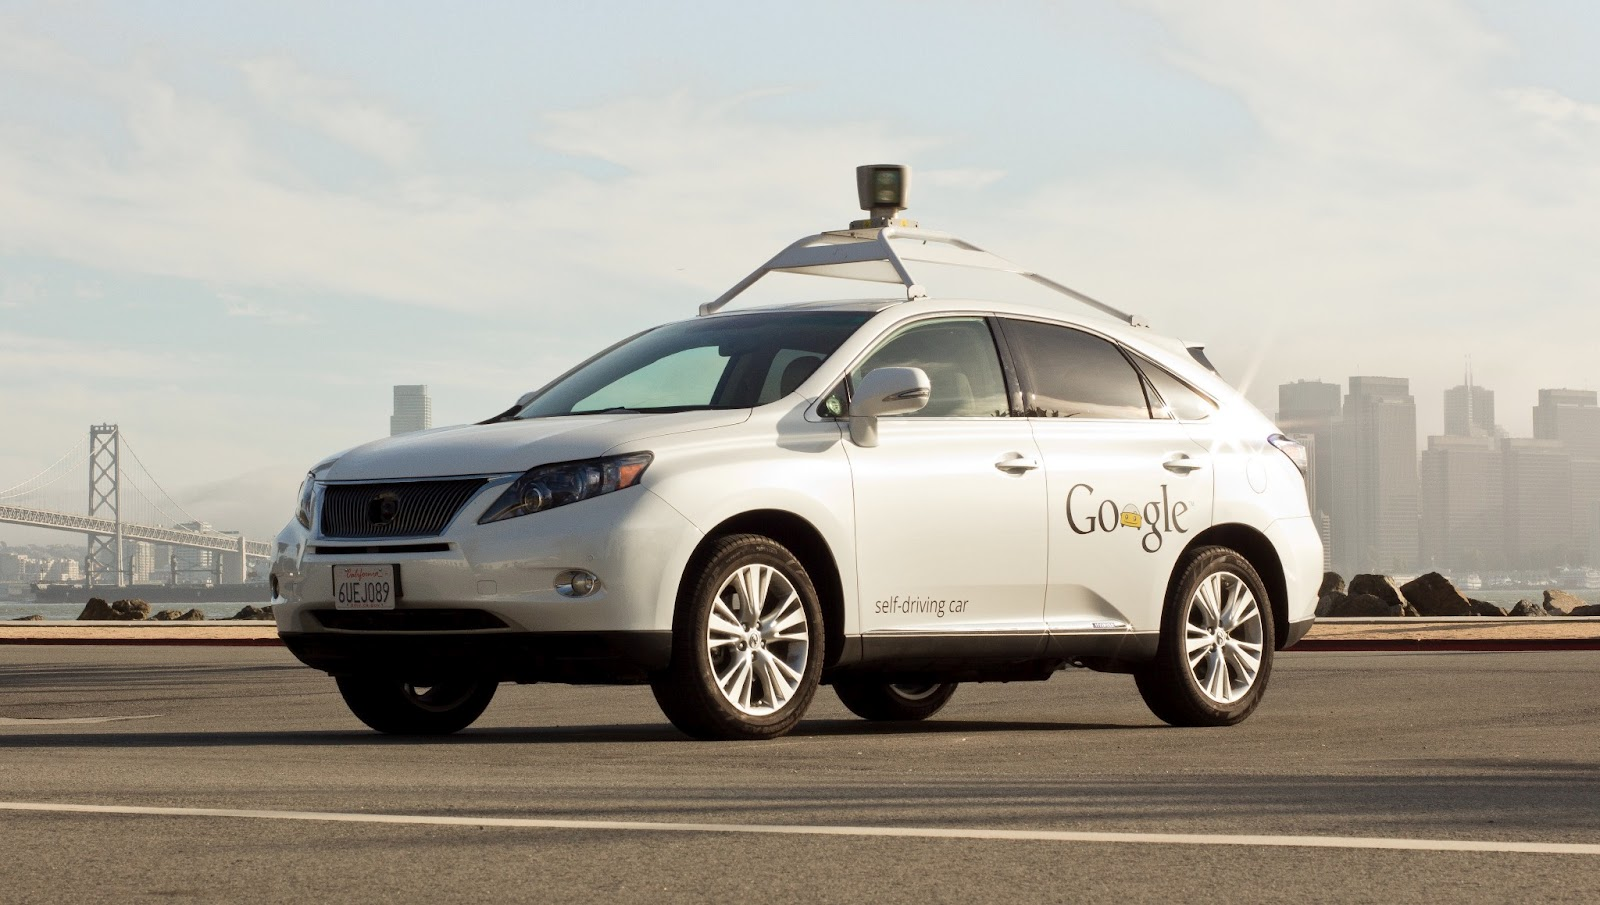
\includegraphics[width=50mm]{img/ch1/Google500KmilesLexus}}
\subfigure[Reconocimiento de caras \tiny{(http://www.netmechanic.co.za/ \copyright)}]{\label{fig:Figure_E}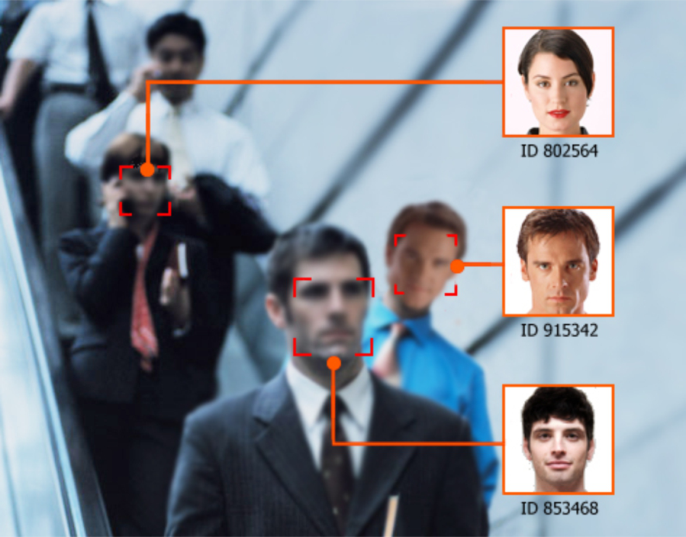
\includegraphics[width=50mm]{img/ch1/face_recognition_technology}}
\caption[Aplicaciones en visión por computador]{Imagenes de aplicaciones en visión por computador }
\label{fig:aplicaciones_vision_por_computador}
\end{figure}


\indent Las diferentes etapas de la cadena de procesamiento en visión por computador constituyen un conjunto extenso de técnicas, algoritmos y métodos provenientes, entre otros, del mundo de procesamiento digital de imágenes y clasificación del área de máquinas de aprendizaje computacional. En cada una de estas etapas además, se emplean diferentes aproximaciones para dar solución al problema que se intenta resolver. La figura \ref{fig:etapas_vision_computador}, es un diagrama general de las distintas etapas que intervienen en un sistema de visión por computador. Una primera etapa consiste en la adquisición de secuencia de imágenes. Las diferentes imágenes del campo de aplicación que se quiere estudiar, son obtenidas mediante algún dispositivo sensor (cámara de vídeo) que transforma una escena del mundo real en una señal electrónica. Las señales son muestreadas y discretizadas para ser convertidas en una matriz de números que representan la escena en un conjunto de imágenes digitalizadas. La etapa de pre-procesamiento se refiere principalmente al mejoramiento de la entrada por medio de técnicas de procesamiento digital de imágenes. Se aplican métodos en el dominio espacial (transformaciones, filtros espaciales, extensión de contraste, procesamiento y ecualización de histogramas, entre otros) y en el dominio de la frecuencia (técnicas basadas en modificar la transformada de \textit{Fourier} de una imagen) para acondicionar las imágenes que permitan resaltar alguna propiedad que requiera la aplicación específica. El proceso de segmentación es una etapa de subdivisión de objetos en una imagen. Se agrupan componentes de una imagen en elementos que tengan alguna característica propia, como forma, color o distribución estadística del color. Un procedimiento similar complementario a la segmentación, es la sustracción del fondo de imagen en una secuencia, esta consiste en modelar el fondo de imagen y sustraer mediante diferentes técnicas los objetos que están sobre ese fondo modelado. La etapa de extracción de características transforma las imágenes de entrada en una representación de elementos característicos agrupados en un vector de propiedades de la imagen o vector característico. Estos vectores sirven de base en la etapa de clasificación o reconocimiento de patrones. 



\begin{figure}[h!]
  \centering
      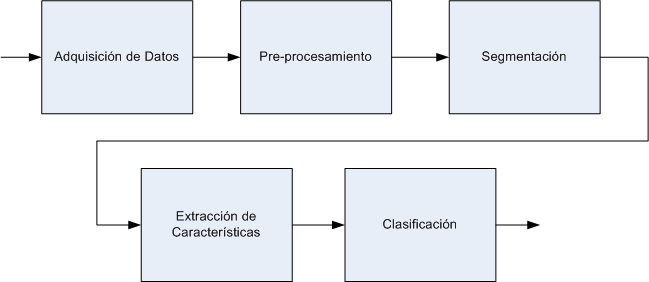
\includegraphics[scale=0.5]{img/ch1/generic_block_diagram_computer_vision}
  \caption[Diagrama de bloques etapas visión por computador]{Diagrama de bloques genérico de las diferentes etapas en visión por computador}
\label{fig:etapas_vision_computador}
\end{figure}

\indent El reconocimiento y clasificación de actividades humanas es una de las tareas más complejas dentro del quehacer de visión por computador, la cual tiene un desarrollo constante dentro de los grupos dedicados a la investigación dentro de este campo. Existe un desafío permanente para desarrollar nuevas técnicas y algoritmos que mejoren los métodos de detección y clasificación de siluetas (``\textit{foreground}'') desde un segundo plano (``\textit{background}'') en una secuencia de imágenes, en diferentes condiciones de iluminación y sombras. Se emplean por ejemplo, algoritmos que construyen un modelo estadístico de los ``píxeles'' de la imagen de fondo, o algoritmos que comparan distribuciones (histogramas) para hacer el seguimiento de objetos en una secuencia de video (``\textit{mean shift tracking}''). 

\indent Se requiere un conjunto preestablecido de imágenes o vídeos, que posibiliten evaluación y comparación de las técnicas y métodos utilizados en segmentación, clasificación y reconocimiento de actividades humanas. En este contexto, existe una variedad de conjuntos de datos (``\textit{datasets}'') disponibles en la comunidad, para ser usados como parte del proceso de evaluación y comparación de algoritmos. Estas base de datos públicas, se componen de imágenes y acciones en secuencia, tomadas desde el mundo real en diferentes ángulos de observación, condiciones ambientales e iluminación.

\indent Los investigadores requieren alguna referencia que les permita evaluar y comparar sus modelos. Deben asegurar que el modelo desarrollado cumple con los objetivos propuesto originalmente. En este ambiente surgen diferentes metodologías de evaluación de modelos, así como los conjuntos de datos que permiten emular un medio ambiente sobre el cual los algoritmos pueden ser ejecutados. 



\indent La finalidad de este trabajo de tesis, consiste en una primera etapa, implementar una plataforma de software que permita, incorporar y evaluar nuevos algoritmos de visión por computador. Es un sistema prototipo de software que pretende establecer una base estándar de evaluación de desempeño de distintos tipos de algoritmos, relevantes en el desarrollo del campo de visión por computador. Este sistema de software viene para ayudar a reducir los tiempos de desarrollos de nuevos algoritmos y evaluar cambios de comportamiento de pequeñas modificaciones en algoritmos desarrollados. Proporciona una infraestructura base para desarrollar y posteriormente evaluar desempeño de nuevos software en visión por computador. Una segunda parte se propone consolidar las métricas de evaluación más utilizadas del campo de clasificación, en una herramienta de software única. Se busca de esta manera, obtener una métrica final de evaluación. El escenario de evaluación utilizado es MuHAVI \cite{singh_muhavi_2010}, un conjunto de datos públicos que dispone diferentes acciones y condiciones orientado a la detección de acciones humanas.


\section{Descripción del problema}
\indent Este trabajo plantea la utilización de un conjunto de datos de reconocimiento de acciones humana “MuHAVI” \cite{singh_muhavi_2010} (``\textit{Multicamera Human Action Video dataset}''), como soporte de comparación y evaluación de rendimiento, de varios algoritmos de sustracción de imágenes de fondo (\textit{Background Subtraction}).  Para esto se propone consolidar un conjunto de métricas de evaluación, utilizadas en clasificación, en una herramienta de software que permita evaluar y comparar las siluetas resultantes de estos algoritmos, con una versión anotada de siluetas que dispone la versión mejorada del conjunto de datos MuHAVI-MAS (``\textit{Manually Annotated Silhouette}'') . 


\indent Se busca adaptar el algoritmo desarrollado por Zezhi Chen \cite{chen_vehicle_2012}, propuesto inicialmente para localización, clasificación y seguimiento de vehículos, y otras versiones equivalentes de sustracción de fondo, en un único sistema de software que incorpore estas diferentes aproximaciones y generar un conjunto total de siluetas de las diferentes secuencias en MuHAVI para evaluar el rendimiento final de cada algoritmo.



\section{Solución propuesta}

\indent Se proyecta desarrollar un sistema de software, basado en un modelo orientado a objetos, que permita evaluar algoritmos de detección y clasificación de actividades humanas. Este software además, implementa e incorpora diferentes versiones de algoritmos de sustracción de fondos, para proporcionar un conjunto de siluetas como resultado final. Facilitando el proceso de evaluación de la herramienta de software principal.

\indent El código implementado para esta solución estará constituido por una biblioteca de clases en C++, que permitiría re-usar su código para diferentes tipos de algoritmos de detección de actividades humanas.

\indent Este trabajo considera varios artefactos de software como entrega final; un sistema de evaluación de algoritmos, un ``framework'' de software que incorpore los diferentes algoritmos de sustracción de fondo, y un conjunto de siluetas necesarias para los algoritmos implementados y otras versiones de estos.

\indent El resultado será un prototipo de software que puede constituir la base para el desarrollo de una plataforma de evaluación de algoritmos empleados en visión por computador.



\section{Objetivos y alcances del proyecto} 
\subsection{Objetivo general}

\indent Implementar un sistema prototipo de software, que incorpore algoritmos de sustracción de fondo empleados en visión por computador, y desarrollar una herramienta de software de evaluación de desempeño para los algoritmos implementados, con el propósito de generar automáticamente siluetas desde conjunto de datos de reconocimiento de acciones humana usando el algoritmo de mejor rendimiento.

\subsection{Objetivos específicos}

\begin{itemize}
\item Implementar el algoritmo de sustracción de fondo propuesto por Zezhi Chen\cite{chen_vehicle_2012} en un programa ejecutable desarrollado en un lenguaje de programación C++ orientados a objeto.
\item Desarrollar un sistema de software base que incorpore otros algoritmos de sustracción de fondo.
\item Implementar una herramienta de software que consolide las métricas más utilizadas en sistemas de clasificación.
\item Evaluar las siluetas resultantes de los distintos algoritmos ejecutados sobre MuHAVI.
\item Generar curvas comparativas del desempeño de los algoritmos.
\item Generar y publicar el conjunto total de siluetas resultantes del algoritmo con mejor desempeño para de todas las secuencias del conjunto de datos MuHAVI 
\end{itemize}


\subsection{Alcances} 

Este trabajo tesis considera varios artefactos como entrega final; desarrollo de un software prototipo que incorpora algoritmos de sustracción de fondo, identificación de métricas de evaluación de calidad, implementación de un programa que evalúa siluetas obtenidas por los distintos algoritmos, un conjunto de siluetas producidas automáticamente, evaluación de desempeño del conjunto de algoritmos de detección de fondo incluidos en el sistema de software prototipo.
El resultado será un prototipo que puede constituir la base para el desarrollo de un ``framework'' de software para evaluación de otros algoritmos de usados en la detección de actividades humanas.


\section{Metodologías y herramientas utilizadas} 

\indent La metodología a utilizar en el desarrollo de este trabajo de tesis, se apoyará en una etapa de investigación, implementación y verificación de resultados. Esta metodología estará basada en las actividades del método científico

\begin{itemize}
\item Identificación del problema. Existe un nuevo método de detección, seguimiento y clasificación de vehículos en autopistas urbanas que podría adaptarse para ser usado en detección de actividades humanas sobre una base de datos denominada MuHAVI.

\item Planteamiento de una hipótesis. Los algoritmos que componen el método Z Chen \cite{chen_vehicle_2012} pueden ser adaptados e implementados para ser usados sobre MuHAVI en la detección de actividades humanas.

\item Revisión de la literatura: Esta etapa consiste en hacer una revisión de las distintas publicaciones que dieron origen a la mejora de este método propuesto por Z Chen \cite{chen_vehicle_2012}. Además, revisar los actuales trabajos de clasificación basado en redes neuronales que permitan reconocimiento de actividades humanas.

\item Implementación del modelo: Se basa en la implementación de los algoritmos de este método en clases C++ basados en el framework de visión por computador ``OpenCV".

\item Etapa de validación y verificación certifica que la implementación realice detección de siluetas y posterior clasificación de estas. Es en esta etapa donde se hará un uso intensivo del software implementado para hacer una clasificación total de MuHAVI.

\item Análisis de resultados y conclusiones, los resultados obtenidos en la etapa anterior son contrastados y comparados para obtener conclusiones sobre el método implementado.
\end{itemize}

\subsubsection{Herramientas de desarrollo}

\begin{itemize}
\item Sistema operativo Linux Ubuntu 12.04
\item Biblioteca de maquinas de aprendizaje y visión por computador OpenCV versión 2.4.4 (``Open Source Computer Vision Library")
\item Compilador GNU C++
\item Sistema de control de versiones "GIT"
\item CMake.
\end{itemize}

\subsubsection{Ambiente de desarrollo}

\indent Es proyecto será realizado en dependencias particulares, se dispondrá de un equipo computacional para hacer el desarrollo de esta aplicación de software.





\section{Resultados obtenidos}

Este trabajo de tesis presenta los siguientes resultados 
\begin{itemize}
\item Un sistema de software base, implementado en lenguaje de programación C++, que permite agregar y utilizar algoritmos de sustracción de imágenes de fondo usados comunmente en el área de visión por computador.
\item Implementación de un algoritmo de basado en mixtura de componente gaussianos, denominado `\textit{Self-Adaptive Gaussian Mixture Model}'  (\textit{SAGMM}).
\item Implementación de una herramienta de software que permite hacer evaluación de desempeño de los resultados obetnidos por algoritmos de sustracción de imágenes de fondo, empleando las métricas más comunes en evaluación de rendimiento.
\item Generación y publicación de siluetas resultantes, utilizando \textit{SAGMM}, de todas las secuencias del conjunto de datos MuHAVI.
\end{itemize}

\section{Organización del documento}

El primer capítulo de este trabajo de titulación se presenta el proyecto a desarrollar, se menciona el alcance, objetivo general, y lo objetivos específicos necesarios para lograr el objetivo general. Se detalla las herramientas necesarias para construir el proyecto, finalmente se hace una breve descripción de la solución propuesta. En segundo capítulo se hace una revisión bibliográfica de los principales temas abordados en la tesis. Se detalla el estado actual de los métodos de sustracción de fondo en la comunidad de investigación en visión por computador, especialmente en los métodos de modelado estadístico. Se mencionan las métricas más utilizadas para evaluar segmentación de imágenes y clasificación de actividades, también se hace una breve mención de los distintos conjunto de datos construidos especialmente para evaluación de algoritmos de detección de actividades. El tercer capítulo se dedica exclusivamente a describir los algoritmos implementados en este trabajo de tesis, se detalla el algoritmo de sustracción de fondo usando mixtura de componentes Gaussianas. El capítulo cuarto describe los métodos empleados para evaluar calidad, y se hace diferencia entre métodos de evaluación subjetiva y objetiva. El quinto capítulo se dedica a mencionar las herramientas, los criterios y las decisiones para llevar a cabo este trabajo de tesis. Se describe también a nivel de bloques las distintas implementaciones de software realizadas, se presentan diagramas UML de paquetes y clases de los sistemas implementados. El sexto capítulo, detalla el resultado de las experimentaciones, y sus análisis, se muestran también las curvas características de resultados. Se agrega un apéndice con gráficas de los resultados obtenidos separados por  por algoritmo. Finalmente el capítulo de las conclusiones, proporciona una idea del resultado general, se hacen las comparaciones de los diferentes algoritmos y se indican los posibles trabajos futuros que se podrían abordar a partir de este trabajo.




\chapter{Estado del Arte}


\indent Los algoritmos de sustracción de fondo (``\textit{Background Subtraction Algorithms}'') modelan esencialmente el segundo plano (``\textit{Background}'') de una imagen con la finalidad de detectar movimiento de objetos (''\textit{Foreground}'') en una secuencia de video. Aplicaciones como vigilancia a través de video, detección de movimiento y clasificación de acciones, necesitan primero modelar la imagen de fondo y luego detectar los objetos móviles.

\indent Modelar el fondo de imagen plantea una serie de desafíos que han sido abordados desde diferentes perspectivas por los investigadores. Cambios de luminosidad, movimientos simultáneos, ambigüedad (imprecisión) sombra y fondo, entre otros, constituyen parte de los problemas que deben superar los algoritmos de sustracción de fondo para detectar y clasificar eventos en una secuencia de imágenes. Se han elaborado en la comunidad variados conjunto de datos (``\textit{Datasets}'') \cite{singh_muhavi_2010, weinland_free_2006, schuldt_recognizing_2004, gross_cmu_2001, gorelick_actions_2007} que emulan escenarios y condiciones con el objetivo de evaluar robustez, rendimiento, calidad en clasificación, de los diferentes modelos de fondo desarrollados. Esta lista de escenarios, es un conjunto de situaciones generales normalmente encontradas en secuencias de video, las cuales constituyen un punto de comparación y referencia entre los diferentes algoritmos implementados en la comunidad. Una descripción más detallada de estas situaciones generales es mencionada en \cite{toyama_wallflower_1999}.

\indent Numerosos métodos de modelado de fondo han sido construidos considerando estas diferentes condiciones. Un estudio publicado por \textit{Bouwmans}\cite{bouwmans_recent_2011} (2011)  presenta un cuadro general de estos métodos y hace una clasificación en diferentes categorías dependiendo de la forma de construir el modelo del fondo. Un modelo básico consiste en usar promedios, medianas o análisis de histogramas en el tiempo. Una técnica simple es calcular el promedio de una escena sin objetos en movimientos, restar nuevos cuadros de esta imagen y comparar a través de un umbral. Otro tipo de modelo se construye basado en distribuciones estadísticas, particularmente en distribuciones del tipo ``\textit{Gaussianas}'', usando variables estadísticas para clasificar los píxeles. Se construyen modelos con redes neuronales en la que una red entrenada podría distinguir entre un píxel perteneciente al fondo o al objeto en movimiento. Otros modelos emplean ``\textit{clusters}'' para agrupar píxeles en diferentes elementos dentro de una secuencia. También existen modelos que emplean filtros especiales para hacer una estimación del fondo, como filtros de ``\textit{Kalman}'' o ``\textit{Tchebychev}''.  

\textit{Bouwmans}\cite{bouwmans_recent_2011} también evidencia un principio de funcionamiento de la mayoría de los métodos de sustracción de fondo, independiente del tipo de modelo e implementación usado. Establece ciertas etapas que se cumplen en los modelos de fondo: modelado de fondo, inicialización del fondo, mantenimiento del fondo, detección (\textit{foreground}), elección de medida de la característica (píxel, block, cluster), elección del tipo de característica (color, borde, texturas).

\section{Modelo de Mixtura de Gaussianas}

\indent Mixtura de Gaussianas (\textit{Gaussian Mixture Model - GMM}) ha sido uno de los métodos más mencionados en la literatura como herramienta de modelo estadístico para obtener el fondo de una secuencia de imágenes. Mixturas finita\cite{mclachlan_finite_2000} de distribuciones es una herramienta de modelado estadístico, análisis de datos e inferencias, usado como base para proporcionar modelos descriptivos de distribuciones en distintas áreas de aplicaciones. Tiene la propiedad (entre otras) de estimar parámetros en un esquema de aprendizaje no-supervisado, de observaciones producidas por un conjunto de fuentes aleatorias. En métodos de sustracción de fondo se utiliza mixtura de Gaussianas para modelar en el tiempo los valores de un píxel (o un vector de valores en espacio de colores RGB) y clasificar en diferentes categorías, generando ``\textit{clusters}'' de píxeles los cuales representan las diferentes mixturas de componentes.
 
\indent Uno de los primeros trabajos realizados con distribuciones estadísticas, que marca el inicio de investigaciones relacionadas con la utilización de mixtura de distribuciones para modelar fondo, es el trabajo de \textit{Friedman} y \textit{Russell} \cite{friedman_image_1997}. Ellos proponen, en un sistema de vigilancia del tráfico automovilístico, obtener el fondo mediante una composición fija de distribuciones Gaussianas. Modelan el valor de intensidad de un píxel con tres distribuciones predeterminadas, asociadas a tres diferentes tipos de objetos: vehículos, sombras, y camino (fondo de la imagen). Utilizan una versión incremental del algoritmo esperanza-maximización\cite{dempster_maximum_1977} (\textit{EM}), para inicializar y actualizar (como mecanismo de aprendizaje no-supervisado) los parámetros de la mixtura del modelo. La clasificación de píxeles es realizada comparando varianza con un umbral definido por la distancia \textit{Mahalanobis}. Durante el proceso de inicialización las tres distribuciones son etiquetadas por una heurística que determina como sombra el componente más oscuro, la distribución de vehículos se relaciona con una mayor varianza, y la distribución del camino con la menor varianza. 

Una aproximación similar es el trabajo de \textit{Stauffer} y \textit{Grimson}\cite{stauffer_adaptive_1999}. Ellos modelan el valor de un píxel con una mixtura de Gaussianas, a diferencia de \textit{Friedman} y \textit{Russell}\cite{friedman_image_1997} que utilizan un conjunto predeterminado de distribuciones para modelar un píxel. Ellos señalan que modelar el fondo mediante un conjunto fijo de distribuciones Gaussianas, el funcionamiento del sistema podría funcionar incorrectamente, con los píxeles que no estén  dentro de las distribuciones prefijadas. En su propuesta plantean, que la persistencia y la varianza de cada Gaussiana en la mixtura, determina las distribuciones que pueden corresponder a la imagen de fondo. Los píxeles que no se ajustan con las Gaussianas del fondo, se consideran parte de elementos en movimiento (\textit{Foreground}) y sólo son parte de éste, cuando existe consistente evidencia para convertirla en una nueva Gaussiana de las mixturas del fondo de imagen. Elementos con desplazamiento lento, por ejemplo, no se incorporan en el fondo debido a que su varianza es mayor con respecto a las varianzas que describen el fondo. Cada píxel es modelado por una mixtura de $K$ Gaussianas (K es una valor entre 3 y 5) y los parámetros se inicializan utilizando un algoritmo \textit{K-Means} (\textit{Friedman} y \textit{Russell}\cite{friedman_image_1997} utilizan un algoritmo EM\cite{dempster_maximum_1977}). Este método además, incorpora dos importante parámetros, que serán utilizados para futuras publicaciones. Formulan una constante de aprendizaje $\alpha$, y $T$ un factor de proporción de los datos que podrían ser considerados parte del fondo. 

\indent La estimación de los parámetros en mixtura de componentes es computacionalmente alta y requiere muchos recursos computacionales, en términos de procesamiento y hardware. Una mejora del algoritmo de mixtura de Gaussianas es presentado por \textit{Zivkovic} y \textit{Heijden} \cite{zivkovic_efficient_2006} (2006). Muestran desde una perspectiva Bayesiana, un criterio de selección en tiempo real, del número adecuado de componentes en un píxel. Esto es, adaptar de manera automática el número de componentes a una escena. Es un algoritmo que estima los parámetros de la mixtura en tiempo real y simultáneamente selecciona el número de Gaussianas, usando una distribución a priori de \textit{Dirichlet}. El número $K$ es adaptado en forma dinámica a la característica de la distribución (multimodalidad) de cada píxel;  un píxel podría estar correctamente descrito por una Gaussiana y otro diferente podría quedar representado por un número mayor de Gaussianas (por ejemplo ondulaciones de en la superficie de un lago). Esta nueva aproximación, se basa en trabajos anteriores \cite{zivkovic_recursive_2004, figueiredo_unsupervised_2002, brand_structure_199} que intentan mejorar los problemas que presentan el algoritmo esperanza-maximización (\textit{EM}) para estimar parámetros de una mixtura (caer en un mínimo local si no es inicializado apropiadamente).  

\indent En el contexto de un sistema de detección, clasificación y seguimiento de vehículos en ciudad  Zezhi Chen \cite{chen_vehicle_2012} (2012) menciona como desventajas, en una mixtura de Gaussianas, la sensibilidad a los cambios bruscos de iluminación, e identificación de sombras móviles producidas por vehículos dentro de una escena. Comenta además, el inconveniente de éste modelo en el uso intensivo de recursos computacionales y el cuidado que requieren la sintonización de sus parámetros. Propone un modelo de mixtura Gaussianas auto-adaptativo, basado en el modelo de \textit{Zivkovic} y \textit{Heijden} \cite{zivkovic_efficient_2006}. Presenta, una tasa de aprendizaje dinámica en tiempo real para mitigar los cambios bruscos de iluminación global y un filtro a nivel de cuadros y píxeles para abordar los problemas de ruido y vibración en las cámaras. Esta tasa dinámica logra buena estimación de la media y varianza en caso de fondos que cambian rápidamente. En caso contrario, la tasa dinámica se aproxima a la constante de aprendizaje original\cite{zivkovic_efficient_2006}.

\indent Un método más flexible para tratar con fondos de imagen dinámicos; fluctuaciones de cámaras, movimientos de las hojas de un árbol, etc. Es el algoritmo de estimación de fondo no-paramétrico propuesto por \textit{Elgammal et al.} \cite{elgammal_nonparametricmodel_2000}. Plantea modelar la función de probabilidad mediante el uso de un ``Kernel'' normal Gaussiano. Este modelo no requiere seleccionar el número de componentes Gaussianas, estiman la función de kernel usando información de historia reciente, con el propósito de capturar cambios rápido en una escena. Sin embargo, una de las mayores desventajas de este modelo, está relacionado con el costo computacional, éste requiere mantener en memoria varios cuadros de una secuencia.


\section{Evaluación de rendimiento}

\indent Las variables mayormente mencionadas en la literatura que miden segmentación, corresponden a las métricas definidas para evaluar rendimiento en sistemas de recuperación de información (\textit{Information Retrieval - IR}). Área que viene de la teoría de clasificación. En algoritmos de sustracción de imágenes de fondo se usan frecuentemente las variables \textit{Precision} y \textit{Recall} \cite{prati_detecting_2003, benezeth_review_2008}, para evaluar la clasificación de los pixeles en una imagen. La combinación de estas dos variables definen además \textit{F-Measure} \cite{herrero_background_2009}, que es una medida global del rendimiento de un algoritmo.

\indent Estas variables se usan principalmente, para un tipo de evaluación estática, en la cual el resultado estimado (de una imagen o secuencia de ellas) es comparado con su versión equivalente anotada (\textit{Ground-Truth}). Método conocido como de discrepancia empírica. En general este tipo de evaluaciones utilizan el promedio de las mediciones de verdadero y falso positivo (\textit{TP} y \textit{FP} respectivamente), a la vez verdadero y falso negativos (\textit{TN} y \textit{FN} respectivamente). Combinaciones de estas mediciones, obtenidas desde una secuencia de imágenes, derivan en variables conocidas como tasa de falsos positivos (\textit{False Positive Rate - FPR}) o tasa de falsos negativos (\textit{False Negative Rate - FNR}) \cite{liu_metrics_2011}. En \cite{prati_detecting_2003} emplean estas variables para construir nuevas medidas de calidad, formulando los conceptos denominados ``buena detección'' (\textit{Good Detection}) y ``buena discriminación'' (\textit{Good Discrimination}) \cite{prati_detecting_2003}. Buena detección, se refiere principalmente a minimizar los falsos negativos (FN) y buena discriminación es minimizar falsos positivos, eso es conseguir un buen compromiso entre las variables de ``Recall'' y ``Precision''.

\indent El algoritmo Wallflower\cite{toyama_wallflower_1999} trabajo del año 1999, propone un nuevo modelo de sustracción y mantenimiento del fondo. Éste consiste de estadísticas asociadas a un modelo del fondo. Definen como metodología de evaluación, un conjunto de 10 obstáculos representativos que un modelo ideal debiera superar: objetos desplazados (\textit{moved objects}), cambios graduales de iluminación (\textit{time of de day}), cambios repentinos de iluminación (\textit{light switch}), variaciones (\textit{waving tree}), camuflaje, algoritmo no entrenado (\textit{bootstrapping}), coloración homogénea (\textit{foreground aperture}), objetos inactivos (\textit{sleeping person}), objetos activos (\textit{waking person}), y sombras (\textit{shadows}). Este trabajo, recomienda aplicar la metodología de evaluación propuesta, en cada uno de los diferentes algoritmos para comparar su rendimiento de clasificación, usando falsos negativos (pixeles no reconocidos dentro de un objeto) y falsos positivos (pixeles identificados erróneamente como fondo) como métricas de evaluación de rendimiento.

\indent Un segundo enfoque de evaluación, intenta cuantificar la percepción visual subjetiva que podría tener un observador independiente del resultado final de segmentación. Se definen los conceptos de precisión espacial y estabilidad temporal \cite{cavallaro_objective_2002} \cite{villegas_perceptually-weighted_2004} como métricas objetivas. La idea es ponderar el resultado de la segmentación de acuerdo con la distancia de los pixeles clasificados (background/foreground) al borde de la imagen segmentada. Mientras mayor es la distancia de un pixel mal clasificado del borde de un objeto, mayor es su ponderación. Para esto se propone, por ejemplo una ponderación del tipo logarítmica para los falsos positivos y una ponderación lineal para falsos negativos \cite{cavallaro_objective_2002} \cite{villegas_perceptually-weighted_2004}. Los falsos negativos son más relevantes a mayor distancia, por esto se ponderan linealmente. En \cite{liu_metrics_2011} proponen una forma similar de evaluación, pero definen una función \emph{sigmoidal} para ponderar ambas variables FP y FN.

\indent En el desafio BMC (\textit{Background Model Challenge}) \cite{park_benchmark_2013}, se plantean una serie de métricas como criterio de evaluación de rendimiento. Para esto  proponen dos tipos de evaluaciones, una que mide \emph{calidad estática} y otra \emph{calidad dinámica}. Para medir calidad estática, piden usar \emph{F-measure} que relaciona Precision y Recall, mesurando el total de estas variables de cada escena, es decir, para cada una de las imágenes de la secuencia se debe obtener F-Measure, promediando el total de todos los valores. También, solicitan medir la relación señal a ruido de cada una de las imágenes en la secuencia (\textit{FSNR}). Las mediciones de calidad dinámica, es un concepto que se refiere se refiere a la percepción de segmentación en el tiempo. Utilizan una métrica denominada ``medida de percepción'' (\textit{perceptual measure-SSIM}), y otra denominada ``D-score''\cite{lallier_testing_2011}.


\section{Conjunto de datos}

\indent Se encuentran disponibles en Internet una amplia variedad de conjuntos de imágenes, para ser utilizados como base de evaluación y comparación de nuevos métodos, en las diferentes áreas visión por computador. Estas base de datos, dependiendo de la realidad, facilitan secuencias en diferentes condiciones y conjuntos más elaborados proporcionan imágenes anotadas (\textit{metadata}). Por ejemplo, existen base de datos de peatones \cite{piotr_pedestrian_2012, ess_depth_2007} para ser usadas en sistemas de asistencia a la conducción de vehículos o sistemas de protección a peatones. Otras como Mobo (\textit{CMU Motion of Body}) \cite{gross_cmu_2001}, creada para investigar la forma de caminar de los seres humanos, lo cual permitiría evaluar algoritmos que permitan identificar a las personas por la forma de caminar.

Para clasificación de acciones humanas, existen en la literatura varios conjuntos estándar. KTH \cite{schuldt_recognizing_2004} es un conjunto de seis acciones humanas diferentes entre ellas, ejecutadas por 25 actores en cuatro ambientes distintos: interior, exterior, exterior con diferentes escalas, exterior con diferentes prendas de vestir. Fue introducida para evaluación de reconocimiento de acciones usando mediciones locales de puntos de interés espacio-temporal (\textit{spatiotemporal interest points - STIPs}). Contiene 598 secuencias de vídeos y 2391 acciones. Cada vídeo tiene un promedio de cuatro segundos de duración.

El conjunto de datos Weizman \cite {gorelick_actions_2007}, fue construido para comprobar robustez de un método detección y clasificación de acciones humanas utilizando el concepto volumen espacio-tiempo. Consiste de 90 secuencias de baja resolución, diez acciones distintas ejecutadas por nueve actores en diferentes escenarios y imagen de fondo. Las imágenes son capturadas por una cámara estática localizada frente a estos actores. 

MuHAVi \cite{singh_muhavi_2010} Es un gran conjunto de acciones humanas recolectados desde ocho ubicaciones diferentes (8 camaras), en un escenario irregular emulando iluminación nocturna de la calle. Contiene 17 clases diferentes de actividades, ejecutado por 14 actores. INRIA XMAS \cite{weinland_free_2006} muy similar a MuHAVI \cite{singh_muhavi_2010}, se compone de 11 actividades cotidianas, por ejemplo, mirar la hora, darse vuelta, o caminar, entre otras. Cada acción es ejecutada en tres oportunidades por dize actores, cinco hombres y cinco mujeres. Una de las característica de este conjunto, se refiere que la posición y dirección de las actividades son realizadas en forma libre por los actores, de esta manera se logra que las actividades sean invariante a la vista (\textit{view-invariance}). 








\chapter{Algoritmos sustracción del fondo}

\section{Introducción}


Esta capítulo hace una presentación de dos algoritmos basados en modelos estadísticos para describir el segundo plano de una secuencia y hacer separación de objetos en movimiento de las imágenes del fondo. Se describe el modelo de \textit{Zivkovic y Heidjen} \cite{zivkovic_efficient_2006} de Mixtura de Gaussianas, el cual constituye la base de la mejora propuesta por \textit{Zezhi Chen} \cite{chen_vehicle_2012}. Estos modelos son los algoritmos sobre los cuales se desarrolla este trabajo de tesis. Ambos han sido incluidos en el desarrollo del sistema de software que permite ejecutar, para luego  comparar y evaluar desempeño sobre las secuencias proporcionadas por MuHAVI. El algoritmo de \textit{Zivkovic y Heidjen} se denomina \textit{MOG} (``\textit{Mixture of Gaussians}'') y el de \textit{Zezhi Chen} \textit{SAGMM} (``\textit{Self-Adaptive Mixture of Gaussians}''). 




\section{Modelo General}

La idea general del proceso de sustracción de fondo, es modelar cada uno de los píxeles de una escena, mediante una función de densidad de probabilidad. Se fundamenta, en la suposición que las imágenes de una escena sin objetos en circulación, tienen un comportamiento regular que puede ser descrito por un modelo estadístico. Un evento por ejemplo, podría ser detectado identificando las partes de la imagen, que no se ajustan con el modelo que describe el fondo. Un nuevo píxel sólo va a ser considerado parte del fondo, si su valor queda completamente descrito por la función de densidad de probabilidad. 


El valor de intensidad en el tiempo de un píxel (o en el transcurso de una secuencia), es utilizado para construir una función de densidad de probabilidad, que corresponde al modelo estadístico que describe el comportamiento del píxel. El modelo, es determinado por una combinación lineal de un conjunto de distribuciones Gaussianas, y por su parte, cada componente es caracterizado por un grupo de parámetros, que identifica los elementos que emergen durante el avance de las imágenes.

\begin{figure}[h!]
  \centering
      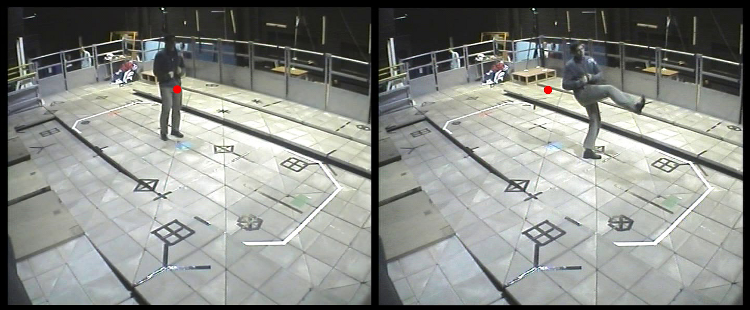
\includegraphics[scale=0.5]{img/figura_3_1}
  \caption[Imágenes 570, 610 de secuencia ``\textit{Kick Camera 3 Person 4}'']{Imágenes 570 y 610 de la secuencia MuHAVI-MAS ``\textit{Kick Camera 3 Person 4}''. El punto en rojo señala la posición de un píxel en dos eventos diferentes}
\label{posicion_340_160}
\end{figure}

\begin{figure}[h!]
  \centering
      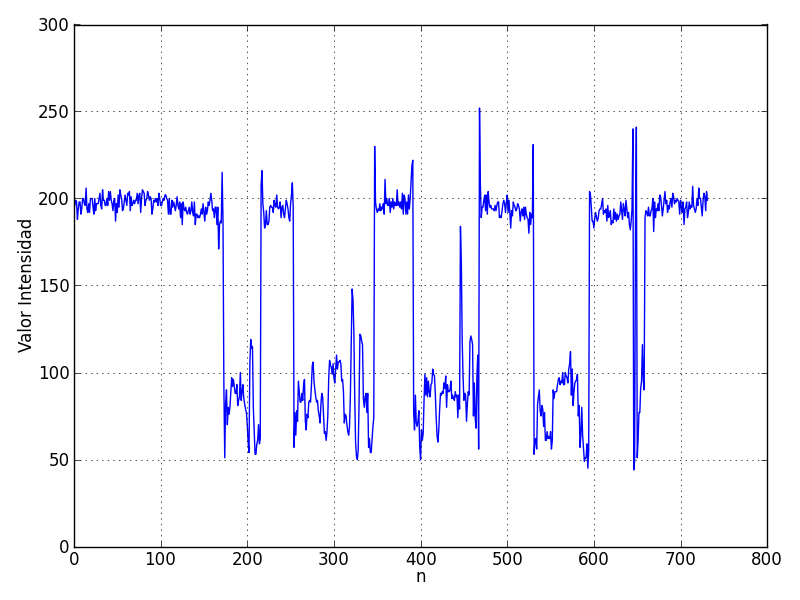
\includegraphics[scale=0.5]{img/figura_3_2}
  \caption[Cambios de intensidad en el tiempo del valor de un pixel ]{Cambios del valor de intensidad de un color en la secuencia completa.}
\label{intensidad_340_160}
\end{figure}


La separación de píxeles entre elementos del fondo y otros objetos, puede ser explicado en forma simple, mediante las dos imágenes de la figura \ref{posicion_340_160}, tomadas de la secuencia MuHAVI \textit{``Kick Camera 3 Person 4''}\cite{singh_muhavi_2010}. Ambas imágenes señalan el estado de un píxel (punto en rojo) en dos momentos diferentes. El píxel indicado en la imagen de la figura \ref{posicion_340_160}(a), es parte en ese instante del actor (\textit{foreground}), ubicado en medio del escenario, y su valor queda determinado por los colores de su vestimenta. Unos segundos después el actor se encuentra en una posición diferente, realizando una determinada acción. En este nuevo instante el valor del píxel queda definido por los colores del escenario (\textit{background}). La gráfica de la secuencia completa (730 imágenes), que describe el comportamiento del píxel se muestra en la figura \ref{intensidad_340_160}. Los cambios repentinos de intensidad (cambio del nivel 200 al rango de valores 50-100), reflejan los pasos del actor en medio del escenario en la posición donde se encuentra localizado este píxel. Por razones computacionales, se asume que los valores de intensidad de los tres componentes en el espacio RGB (azul, verde y rojo) tienen la misma varianza \cite{zivkovic_efficient_2006}, de esta manera la matriz de covarianza queda definida como una matriz identidad multiplicado por ese único valor de varianza.

\begin{figure}[h!]
  \centering
      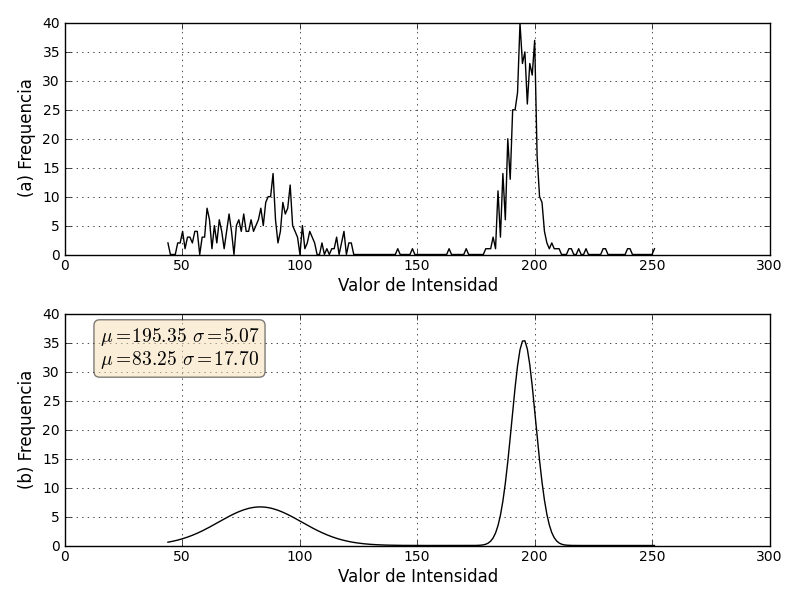
\includegraphics[scale=0.75]{img/histograma_pixel_340_160_3_2}
  \caption[Histograma secuencia completa ``\textit{Kick Camera 3 Person 4}'']{Histograma secuencia completa ``\textit{Kick Camera 3 Person 4}''}
\label{histograma}
\end{figure}

Al observar el rango valores asociados al escenario en la figura \ref{intensidad_340_160}, se evidencian valores más constantes (o menor dispersión) que los del actor cuando pasa por este píxel. Esto también se puede apreciar en el modelo de la secuencia completa que describe el histograma de la figura ~\ref{histograma}(a). En esta imagen se pueden distinguir dos curvas bien definidas, el fondo de imagen y el el actor en movimiento. La mixtura en este ejemplo, se construye ajustando la función de densidad a dos distribuciones Gaussianas, figura (\ref{histograma})(b). De esta manera, el modelo que describe este píxel en particular para esta secuencia, queda completamente definido por una composición de dos funciones Gaussianas. Se puede ver también en esta figura, que la imagen de fondo puede ser asociada con la componente de menor varianza, debido principalmente a la menor dispersión de valores del fondo. Sin embargo, el menor valor de frecuencia puede ser relacionado con el actor en movimiento, debido al menor tiempo que éste cruza el escenario. 

Se aprovecha estas características de la Mixtura de Gaussianas, para hacer una separación entre \textit{foreground} y \textit{background}. Así cuando la componente Gaussiana que describe algún píxel no se ajuste a la distribución con menor varianza, será considerando parte de un objeto en movimiento. No obstante, si este mismo objeto queda estático por un tiempo considerable, la varianza de su distribución Gaussiana comenzará a disminuir y tomar más relevancia (mayor ponderación relativa) que la varianza del componente del fondo, hasta llegar un momento que será considerado parte del fondo de imagen.




\begin{figure}[h!]
  \centering
      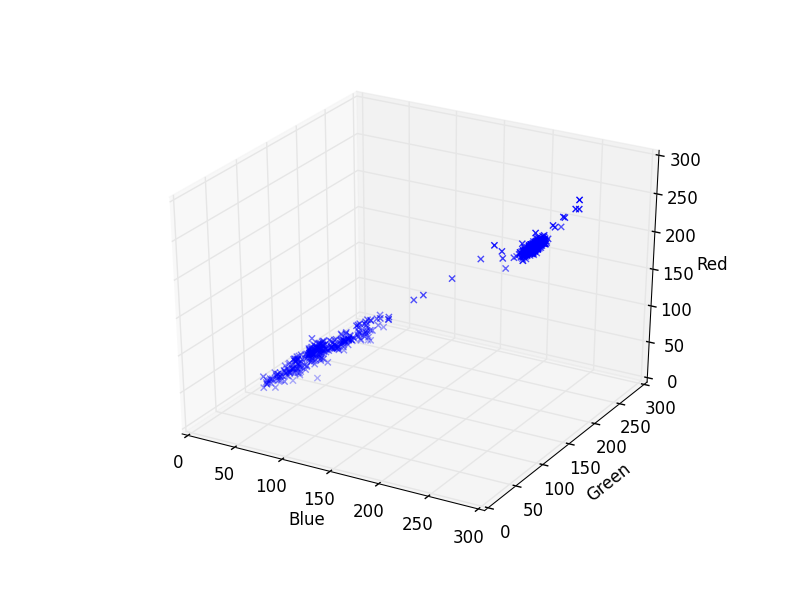
\includegraphics[scale=0.75]{img/scatter_pt_340_160_3D_Blue_Green_Red}
  \caption[Gráfico dispersión 3D secuencia completa ``\textit{Kick Camera 3 Person 4}'']{Gráfico de dispersión en secuencia ``\textit{Kick Camera 3 Person 4}'' que muestra la nube de puntos relacionados con el escenario y el actor en movimiento.}
\label{scatter_3D}
\end{figure}

\begin{figure}[h!]
  \centering
      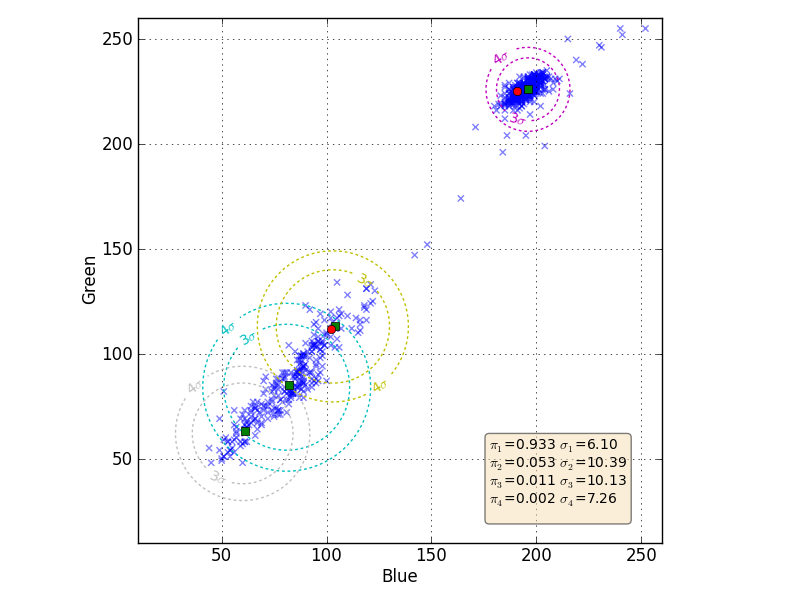
\includegraphics[scale=0.75]{img/scatter_pt_340_160_isotropic_Blue_Green}
  \caption[Gráfico dispersión 2D secuencia completa ``\textit{Kick Camera 3 Person 4}'']{Gráfico de dispersión secuencia ``\textit{Kick Camera 3 Person 4}'', que muestra dos \textit{cluster} bien definidos}
\label{scatter_2D}
\end{figure}

Los gráficos de las figuras \ref{scatter_3D} y \ref{scatter_2D} sirven de ejemplo para entender el procedimiento de actualización de parámetros, de los diferentes componentes Gaussianos definidos en el algoritmo. Estas figuras son gráficos de dispersión de la secuencia completa (\textit{Kick Camera 3 Person 4}) para el mismo píxel del ejemplo señalado en la figura \ref{posicion_340_160}. La dispersión en la gráfica \ref{scatter_3D}, conforma principalmente dos nubes o \textit{clusters} que se asocian con los dos elementos principales de la secuencia: el escenario y las acciones del actor. El \textit{cluster} más compacto de puntos, localizado en el rango 150-250 de los tres ejes de colores, resume los diferentes tiempos que el píxel fue parte del escenario, mientras el otro \textit{cluster} localizado en la parte inferior refleja la cantidad de veces que el píxel fue parte del actor durante sus movimientos.  

Durante el tiempo que dura la ejecución del algoritmo, los componentes Gaussianos de un píxel van siendo creados o suprimidos en tiempo real, dependiendo exclusivamente de los nuevos valores de entrada y el tiempo de permanencia de estos valores, en alguno de los diferentes \textit{clusters} de la secuencia. Los valores presentan un comportamiento dinámico en directa relación con los eventos de la secuencia; éstos se pueden mover entre \textit{clusters} o bien mantenerse en uno de ellos por un largo periodo. Se aprovecha esta división de \textit{clusters} para hacer la separación entre \textit{background} y \textit{foreground}. La gráfica de la figura \ref{scatter_2D} (dispersión verde-azul) destaca cuatro componentes (\textit{clusters}) definidos por el algoritmo, en el instante que el actor se encuentra detenido de pie en medio del escenario, ejemplo de la figura \ref{posicion_340_160}(a). Los dos puntos en rojo revelan la posición del píxel en los \textit{clusters} para las dos imágenes de ejemplo en la figura \ref{posicion_340_160}. Cada uno de estos componentes tiene un factor de ponderación $\pi_k$ que indica el tiempo de permanencia del píxel en la nube de puntos. Este factor de ponderación es incrementado en la medida que el valor del píxel se mantenga dentro de un margen (de uno de los componentes), determinado por la distancia de Mahalanobis, del punto hacia cada uno de los \textit{clusters}. Para discriminar que el píxel es parte del actor (o el escenario), el algoritmo calcula las distancias del pixel a los ``centroides'' (media) de los diferentes \textit{clusters} establecidos en ese instante. El punto es asociado con algún \textit{cluster}, si el resultado de la distancia de Mahalanobis es menor a tres veces su varianza. Si el punto no es vinculado a ninguno de los clusters definidos en ese momento, el algoritmo crea uno nuevo y deja el punto ligado con este nuevo cluster. Una vez que el algoritmo ha identificado el punto en alguno de los clusters, se realiza la clasificación, ya sea \textit{background}  o \textit{foregorund} y por lo tanto el píxel queda clasificado por la característica del cluster, al que ha sido asociado. Esto es, si el cluster en particular tiene un factor de ponderación más alto que todos los demas, ese cluster es \textit{background} y en consecuencia el píxel también. En caso contrario, el píxel que pertenece a un cluster con factor de ponderación inferior, por lo tanto es algún objeto en movimiento.




\section{Mixtura de distribuciones Gaussianas - GMM}


La superposición de distribuciones Gaussianas que describen el comportamiento de un pixel, se define en la ecuación \eqref{eq:mixturegaussians}. Esta es una sumatoria de \textit{``K''} componentes Gaussianos $\mathcal{N}( x | \mu_k , \Sigma_k)$, cada uno ponderado por un factor multiplicativo $\pi_k$, que establece una función de densidad de probabilidad general para el píxel $p(x)$. El factor de ponderación $\pi_k$, es el grado de influencia de cada componente en el comportamiento global del píxel que esta siendo modelado. Los valores de ponderación pueden ser interpretados, como probabilidades de ocurrencias de las diferentes clases, \textit{Background} y \textit{Foreground}, representadas por los diferentes componentes Gaussianos; por ejemplo, $\pi_1$ podría representar la probabilidad que un píxel sea la imagen de fondo. La suma total de los factores $\pi_k$ es 1, indicado en la ecuación \eqref{eq:mixturefactor}. 

\begin{equation} \label{eq:mixturegaussians}
p(x) = \sum_{k=1}^{K} \pi_k \mathcal{N}( x | \mu_k , \Sigma_k)
\end{equation}

\begin{equation} \label{eq:mixturefactor}
\sum_{k=1}^{K} \pi_k = 1
\end{equation}


Una de las principales tareas del algoritmo que implementa mixtura de Gaussianas, es mantener actualizado los $K$ valores estimados de media ($\mu_1, ..., \mu_k$),  covarianza ($\Sigma_1, ..., \Sigma_k$) y el factor de ponderación ($\pi_1, ..., \pi_k$), por cada píxel de una nueva entrada. Se utilizan los valores de intensidad en el espacio de colores RGB, para construir la mixtura de componentes Gaussianas de un píxel.

La estimación de los parámetros $\vec{\theta} = \{\pi_1,..,\pi_k, \mu_1,..,\mu_k,\Sigma_1,..,\Sigma_k \} $ de las distintas mixturas se realiza mediante el método de Máxima Verosimilitud (\textit{Maximum Likelihood Estimate - MLE}). De esta manera, los parámetros estimados por máxima verosimilitud de un conjunto $t$ de muestras $\mathcal{X} = \{\vec{x}^{(1)}, ..., \vec{x}^{(t)}\}$, quedan determinados por la ecuación (~\ref{eq:maxima_verosimilutd}). Una explicación bien detallada de estimación mediante el método de máxima verosimilitud se puede ver en el capítulo 3 de la referencia \cite{duda_pattern_2000}.

\begin{equation} \label{eq:maxima_verosimilutd}
\hat{\vec{\theta}} = arg \max_{\vec{\theta}}  (\log p(\mathcal{X};\vec{\theta}))
\end{equation}

 
Debido a la dificultad de encontrar una solución analítica de \textit{MLE}, se emplea una aproximación numérica iterativa para maximizar la función de verosimilitud.  El algoritmo de esperanza-maximización (EM) \cite{dempster_maximum_1977}, se usa para encontrar soluciones de máxima verosimilitudes. Este es un procedimiento iterativo que busca un máximo local de la función log-verosimilitud. Este algoritmo es fácil de implementar, sin embargo una de sus limitaciones está en la posibilidad de converger en un máximo local no inicializado apropiadamente.


\subsection{Actualización parámetros del Algoritmo}

Esta parte, describe el método de actualización recursivo que se utiliza en la estimación de los parámetros ($\mu_k$, $\Sigma_k$, $\pi_k$) de cada componente Gaussiano, establecido por \textit{Zivkovic y Heidjen} \cite{zivkovic_efficient_2006}. Por razones computacionales, las matrices de covarianza son consideradas Isotrópicas, es decir la matriz de identidad multiplicado por un único valor de varianza.

El modelo del fondo, es estimado desde un conjunto ``$X$'' de entrenamiento, el cuál mantiene una historia específica de muestras por cada píxel. Para adecuarse a los posibles cambios que puedan producirse, las muestras en este conjunto se actualizan constantemente con nuevas entradas y simultáneamente las más antiguas son eliminadas. Un periodo de adaptación ``$T$'' (100 cuadros) es elegido para mantener la historia más reciente del fondo, y en el instante ``$t$'' se tiene el conjunto de entrenamiento $\mathcal{X_T} = \{x^{(t)}, ..., x^{(t-T)}\}$, desde el cual se estima la función de densidad del fondo.

La parte central del algoritmo, consiste en actualizar constantemente los parámetros $\vec{\theta}$ de las distribuciones Gaussianas, que describen el estado de cada píxel en un momento determinado. Las ecuaciones recursivas para estimar los parámetros de una muestra nueva $x^{(t)}$ en tiempo $t$ se presentan a continuación:


\begin{equation} \label{eq:mixturefactor_update}
\hat{\pi}_k \leftarrow  \hat{\pi}_k + \alpha(o^{(t)}_k - \hat{\pi}_k) - \alpha C_T
\end{equation}
\begin{equation} \label{eq:mixturemu_update}
\hat{\vec{\mu}}_k \leftarrow \hat{\vec{\mu}}_k + o^{(t)}_k (\alpha/\hat{\pi}_k) \vec{\delta}_k
\end{equation}
\begin{equation} \label{eq:mixturesigma_update}
\hat{\sigma}^2_k \leftarrow \hat{\sigma}^2_k + o^{(t)}_k (\alpha/\hat{\pi}_k) (\vec{\delta}^T_k \vec{\delta}_k - \hat{\sigma}^2_k)
\end{equation}
\begin{equation} \label{eq:mahalanobis_distance}
D^{2}_{k}(\vec{x}^{(t)})=\vec{\delta}^T\vec{\delta}_k/\hat{\sigma}^{2}_k
\end{equation}

\[
\vec{\delta}_k = \vec{x}^{(t)} - \hat{\vec{\mu}}_k
\]


El factor constante $\alpha$, define una curva de decaimiento exponencial para limitar la influencia de los datos más antiguos. Se usa esta constante, como reemplazo de $T$ mencionado anteriormente, relacionando ambas constante por la siguiente relación: $\alpha=1/T$. 

El algoritmo mantiene un conjunto dinámico de componentes por cada píxel, esto significa que el número de componentes del modelo es diferente en periodos distintos de la secuencia. Se determina que una nueva muestra es cercana con algunos de los componentes si la distancia de \textit{Mahalanobis} \eqref{eq:mahalanobis_distance} es por ejemplo, menor que tres. Fijando el valor del \textit{ownership} $o^{(t)}_k$ en uno si la muestra es cercana y en cero para el caso contrario. Si la muestra no es cercana a alguno de los componentes ($o^{(t)}_k=0$), se crea uno nuevo con los siguientes valores por defecto $\pi_{k+1} = \alpha$, $\hat{\vec{\mu}}_{k+1}=\vec{x}^{(t)}$ y $\hat{\sigma}_{k+1}=\sigma_0$, con $\sigma_0$ un valor de inicialización de la varianza fijado en el algoritmo.

Este algoritmo representa también los diferentes elementos que surgen en la secuencia, como un conjunto de \textit{clusters} en tiempo real. Un nuevo objeto que ingresa en la secuencia se caracteriza por un \textit{cluster} adicional con un valor de ponderación $\pi_k$ muy inferior a los otros componentes. 

Para determinar el píxel como una imagen de fondo, se ordena los factores de ponderación en forma descendente, y los $B$ \textit{clusters} con mayor ponderación se aproximan al modelo del fondo como se indica en la siguiente ecuación.

\begin{equation} \label{eq:clusters}
B=arg \max_{b}  (\sum_{k=1}^{b} \hat{\pi}_k > (1 - c_f))
\end{equation}

El parámetro $c_f$ es un criterio de medición que indica la cantidad de los datos que pueden ser considerados objetos de \textit{foreground} sin la influencia del modelo de \textit{background}. De esta forma si un nuevo objeto se mantiene estático durante algún tiempo, este será presentado como un \textit{cluster} adicional, y su factor de ponderación $\pi_{k+1}$ será incrementado en la medida que se mantenga estático. Sí se mantiene lo suficiente, y el factor $\pi_{k+1}$ supera $c_f$, entonces este objeto puede ser considerado parte del fondo.


\section{Modelo Mixtura de Gaussianas auto-adaptativo}

Este método se origina en un contexto de vigilancia de tráfico en ciudad. Es el resultado de un sistema de detección y clasificación automática de vehículos \cite{chen_vehicle_2012}, que utiliza una variante del método de mixtura de Gaussianas\cite{zivkovic_efficient_2006}, para hacer una separación entre vehículos en circulación y su pista. La modificación propuesta aborda el problema de cambios bruscos en la iluminación, que podrían transformar todo el segundo plano (\textit{background}) de la imagen, en primer plano (\textit{foreground}). Además, la tasa normal de aprendizaje se transforma en una tasa dinámica en tiempo real. Se intenta con esta modificación, obtener una tasa que se adapte en forma dinámica a los cambios de iluminación. También se utiliza como método de procesamiento previo, un filtro espacial y temporal\cite{chen_background_2009} para compensar las alteraciones producidas por vibraciones de las camaras. Finalmente para afrontar el problema de cambios en iluminación local, como sombras y reflexiones de luz, modifican un algoritmo de extracción de sombras \cite{horprasert_astatistical_1999}, para incorporar el factor de iluminación global.


\subsection{Factor de iluminación global}
En \cite{chen_self-adaptive_2011}, se menciona el modelo de detección de cambio invariante a iluminación (\textit{ICDM}), al proceso que determina el factor de cambio de iluminación global.  Éste es un procedimiento que realiza el cociente uno a uno entre un conjunto ``$s$'' de pixeles de una imagen de entrada ($i_c$) y su imagen de referencia ($i_r$). El factor de iluminación global ``$g$'' se determina como la mediana de todas las divisiones resultantes, ``\textit{Median of Quotient (MofQ)}''.

\begin{equation} \label{eq:mofq}
g = \median_{(s \in S)}  \left(\frac{i_{r,s}}{i_{c,s}}\right)
\end{equation}

Se define además un contador ``$c_k$'' por cada componente Gaussiano en la mixtura. Este contador se utiliza para mantener un registro de cuantos puntos han contribuido en la estimación de parámetros de cada Gaussiana, cada vez que los parámetros de un componente Gaussiano es actualizado, el contador también es incrementado. En caso que un nuevo componente se agrega a la mixtura este contador es inicializado a uno. 

El factor de aprendizaje $\alpha$ es usado como base para construir un nuevo factor de aprendizaje $\beta$, el cual utiliza el contador de componentes Gaussianas mencionado anteriormente. Las nuevas ecuaciones de actualización de parámetros se detallan a continuación:


\begin{equation} \label{eq:sagmm_betha}
\beta_k = \alpha(h + c_k)/c_k
\end{equation}

\begin{equation} \label{eq:sagmm_mu}
\hat{\vec{\mu}}_k \leftarrow \hat{\vec{\mu}}_k + o^{(t)}_k (\beta/\hat{\pi}_k) \vec{\delta}_k
\end{equation}

\begin{equation} \label{eq:sagmm_sigma}
\hat{\sigma}^2_k \leftarrow \hat{\sigma}^2_k + o^{(t)}_k (\beta/\hat{\pi}_k) (\vec{\delta}^T_k \vec{\delta}_k - \hat{\sigma}^2_k)
\end{equation}

\begin{equation} \label{eq:sagmm_ck}
c_k \leftarrow c_k + 1
\end{equation}

\begin{equation} \label{eq:sagmm_delta}
\hat{\vec{\delta}}_k = g \bullet \vec{x}^{t} - \hat{\vec{\mu}}_k
\end{equation}

Si el valor de un pixel de la imagen de fondo varia muy rápidamente, el valor del contador $c_k$ para ese píxel no será muy grande, por lo que el valor de $\beta$ aumentará. Actualizando de esta manera el fondo más rápidamente. Por otra parte si el fondo es muy estable, el valor se $\beta$ se aproximará a $\alpha$. También se observa que la distancia de Mahalanobis es balanceada por el factor de cambio de iluminación global $g$.


\subsection{Filtro espacial y temporal}
Este filtro que prepara la imagen antes de ser procesada por el método modificado de mixturas. Realiza un suavizado de cada componente espectral. En una imagen se habla de dominio espacial para referirse a los píxeles localizados en la matriz de valores y dominio espectral para los componentes de frecuencia obtenidos después de aplicar la transformada de Fourier. El domino espacial se relaciona con el dominio espectral, por medio del teorema de la \textit{convolución}. La convolución (descripción muy básica), es el proceso mover una mascara o kernel píxel a píxel sobre una imagen y obtener un resultado de cada píxel de acuerdo con los coeficientes de la mascara. Los filtros del tipo Gaussiano, tienen la particularidad que en ambos espacios (espacial y espectral) son representados por una función Gaussiana.


\begin{equation} \label{eq:sagmm_filter}
K_{h_s,h_s} = \frac{C}{h_s h_t} k \left( {\| \frac{x^s}{h_s} \|}^2 \right) k \left( {\| \frac{x^t}{h_t} \|}^2 \right)
\end{equation}

$C$ es una constante de normalización, $x^s$ es la parte espacial y $x^t$ la parte temporal, $k(x)$ es un perfil común de kernel (Gaussiano) usado en ambos dominios, temporal y espacial. Las variable $h_s$ y $h_t$ son el ancho de banda de los kernels. 


\begin{figure}[h!]
\centering
\fbox{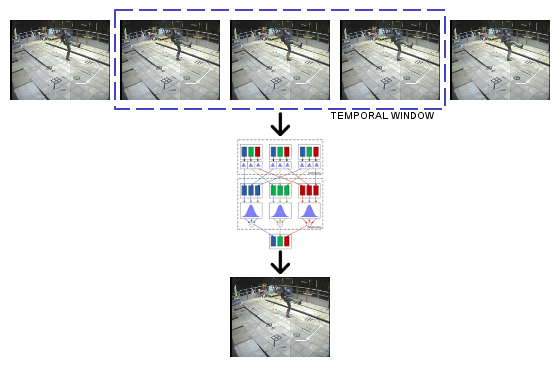
\includegraphics[scale=0.5]{img/Spatio_Temporal_Filter_Example}}
\caption[Procesamiento temporal de tres imágenes]{Procesamiento temporal de tres imágenes de una secuencia.}
\label{fig:spatio_temporal_filter_example}
\end{figure}


La figura \ref{fig:spatio_temporal_filter_example} es un ejemplo del funcionamiento de este filtro. Se define una ventana temporal que define el número de imágenes que serán procesadas simultáneamente por este filtro. La entrada del filtro, es el número de imágenes que mantiene la ventana temporal, y su salida es la imagen filtrada que será la nueva entrada del algoritmo. Esta ventana puede ser visualizada como un marco que se desliza sobre la secuencia y entrega una imagen procesada como salida.

\begin{figure}[h!]
\centering
%\subfigure{%\documentclass{article}
\documentclass[preview]{standalone}
%\usepackage{tikz}
\usepackage{pgfplots}
%\usepackage{subfigure}

\begin{document}

\newcommand\gauss[2]{1/(#2*sqrt(2*pi))*exp(-((x-#1)^2)/(2*#2^2))} 
\tikzstyle{place}=[circle,draw=blue!50,fill=blue!20,thick]


\begin{tikzpicture}[scale=0.5,cube/.style={very thin,black}]
    %\draw[step=1cm,gray,very thin] (-2,-2) grid (24,24);

    \node[inner sep=0cm] (gaussian) at (2.75,7.5)
        {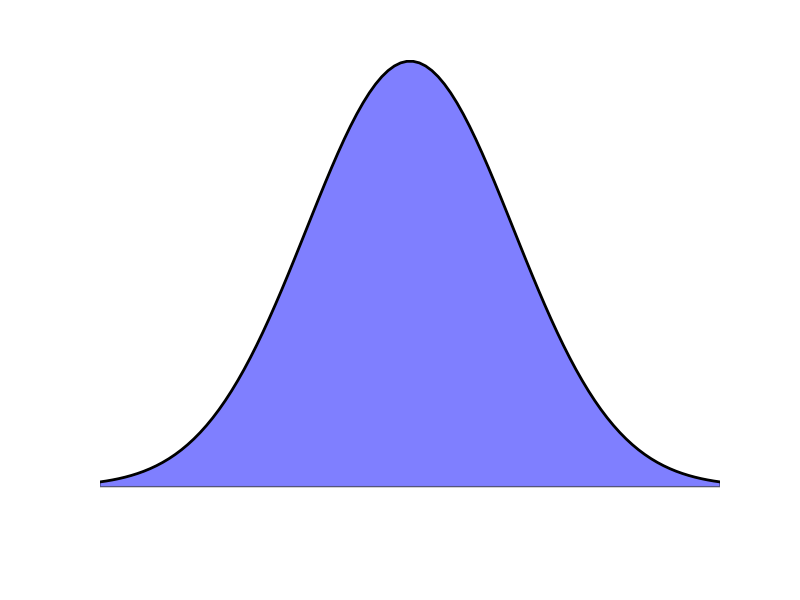
\includegraphics[width=.14\textwidth]{gaussian.png}};
    \node[inner sep=0cm] (gaussian) at (6.75,7.5)
        {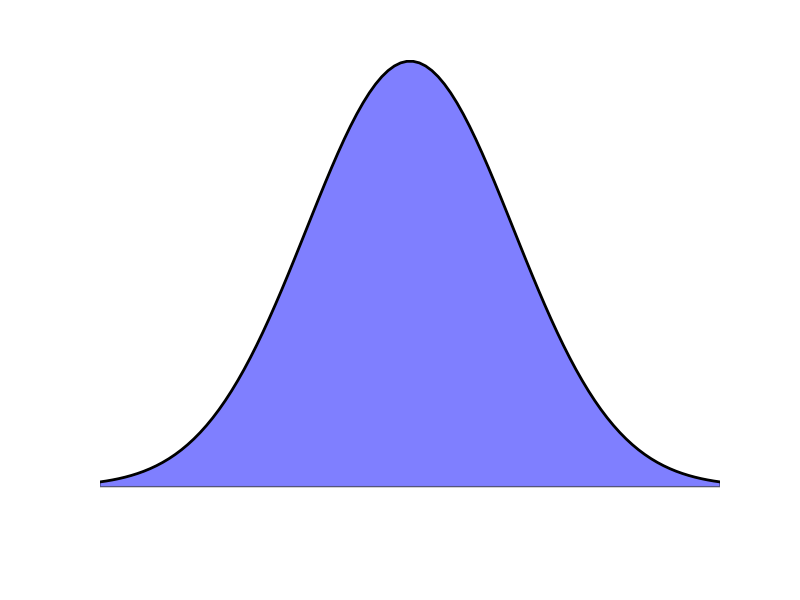
\includegraphics[width=.14\textwidth]{gaussian.png}};
    \node[inner sep=0cm] (gaussian) at (10.75,7.5)
        {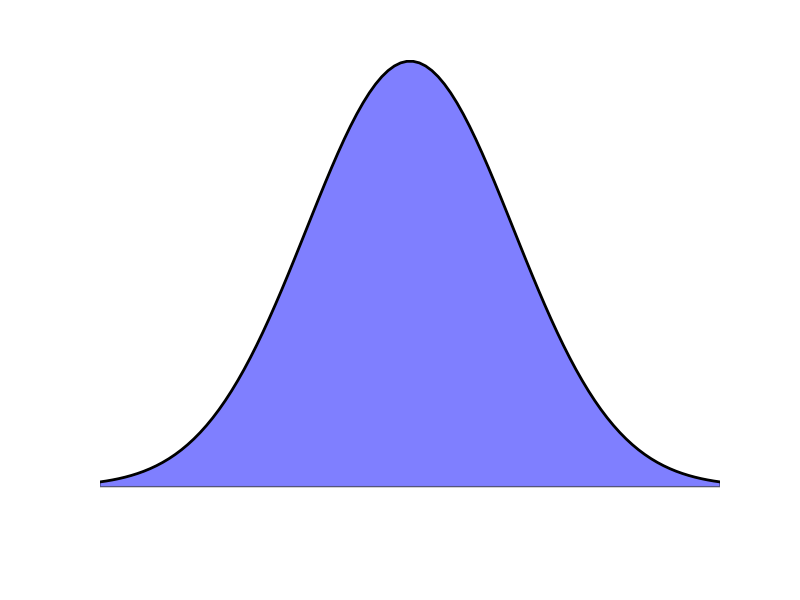
\includegraphics[width=.14\textwidth]{gaussian.png}};

    \node[inner sep=0cm] (gaussian) at (1.5,17.5)
        {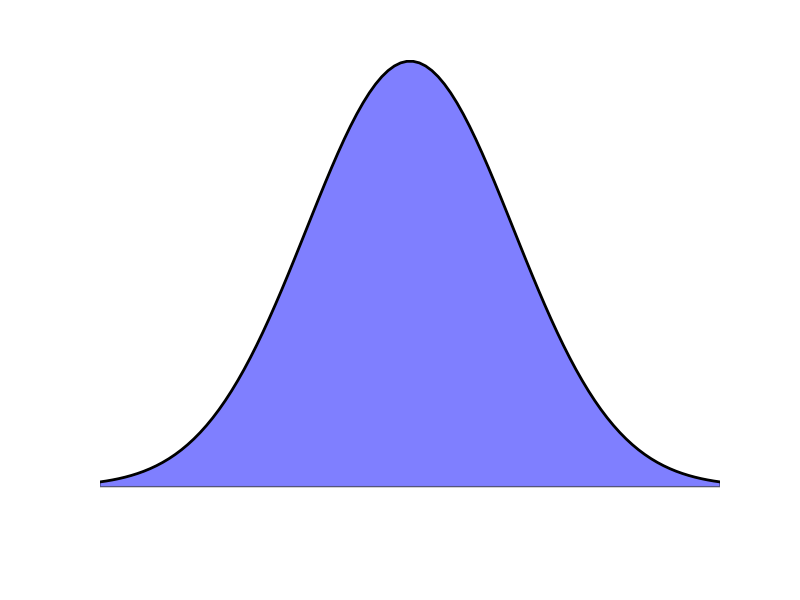
\includegraphics[width=.05\textwidth]{gaussian.png}};
    \node[inner sep=0cm] (gaussian) at (2.5,17.5)
        {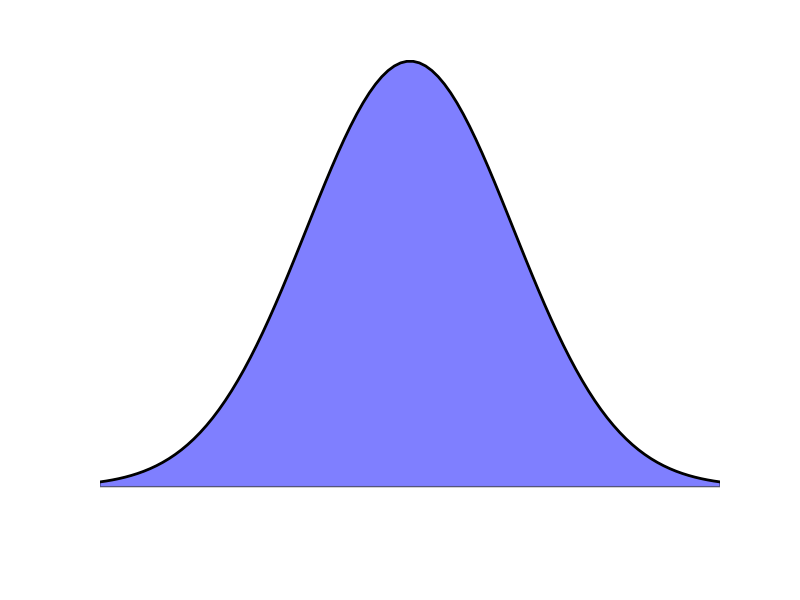
\includegraphics[width=.05\textwidth]{gaussian.png}};
    \node[inner sep=0cm] (gaussian) at (3.5,17.5)
        {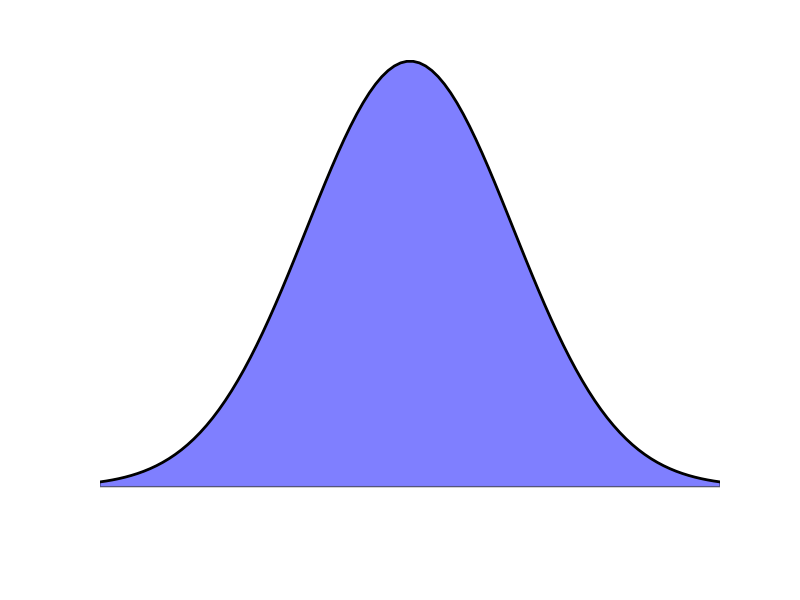
\includegraphics[width=.05\textwidth]{gaussian.png}};

    \node[inner sep=0cm] (gaussian) at (5.5,17.5)
        {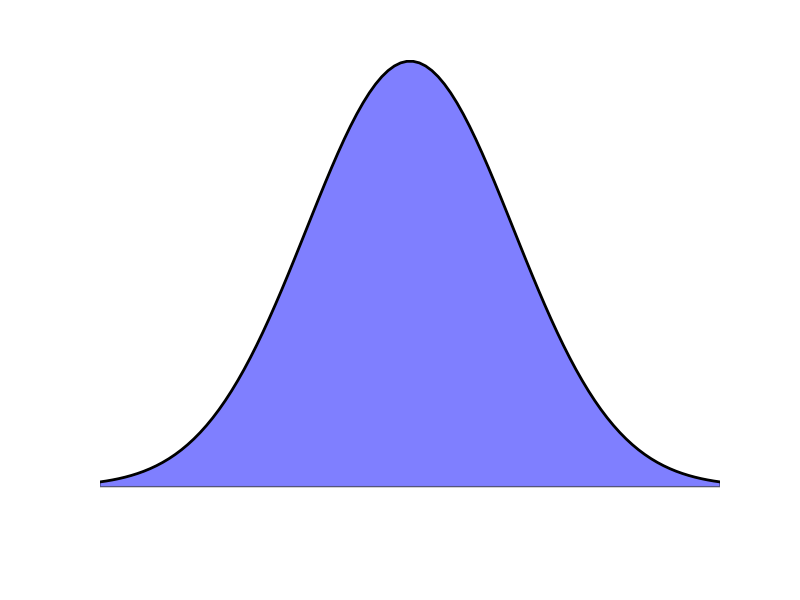
\includegraphics[width=.05\textwidth]{gaussian.png}};
    \node[inner sep=0cm] (gaussian) at (6.5,17.5)
        {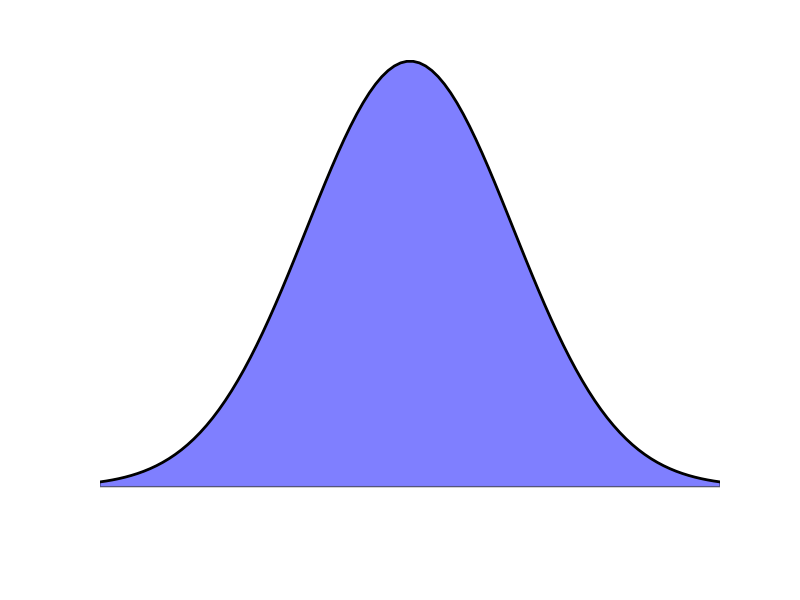
\includegraphics[width=.05\textwidth]{gaussian.png}};
    \node[inner sep=0cm] (gaussian) at (7.5,17.5)
        {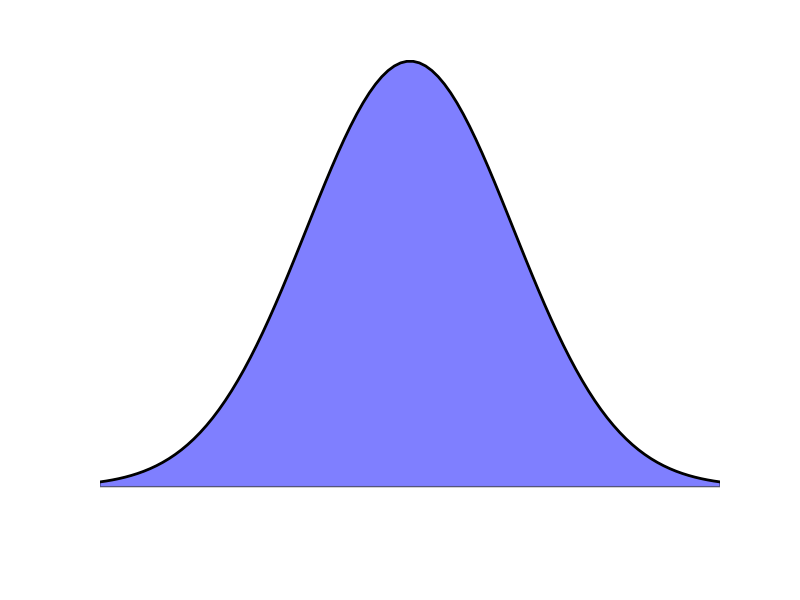
\includegraphics[width=.05\textwidth]{gaussian.png}};

    \node[inner sep=0cm] (gaussian) at (9.5,17.5)
        {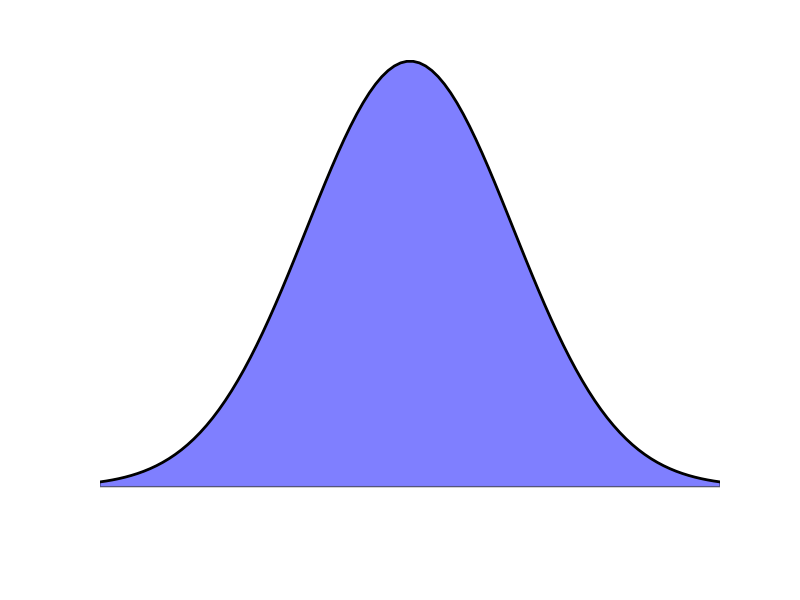
\includegraphics[width=.05\textwidth]{gaussian.png}};
    \node[inner sep=0cm] (gaussian) at (10.5,17.5)
        {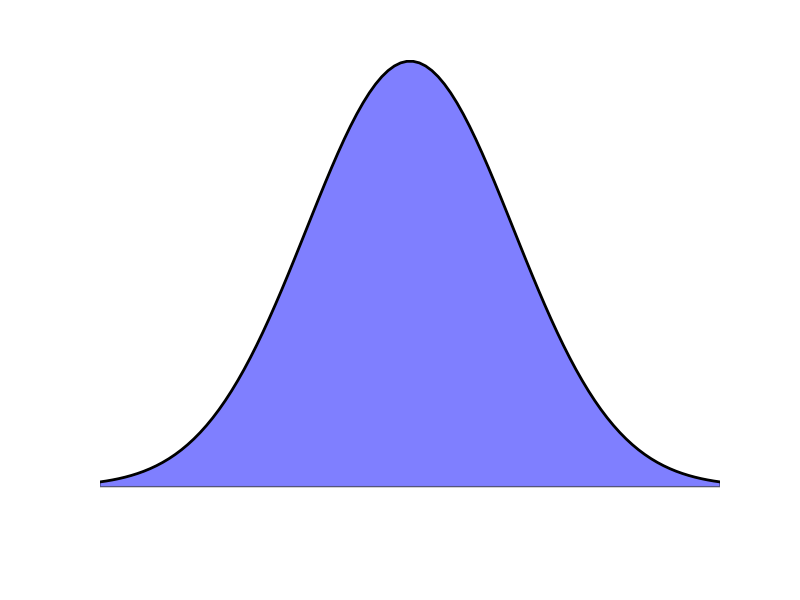
\includegraphics[width=.05\textwidth]{gaussian.png}};
    \node[inner sep=0cm] (gaussian) at (11.5,17.5)
        {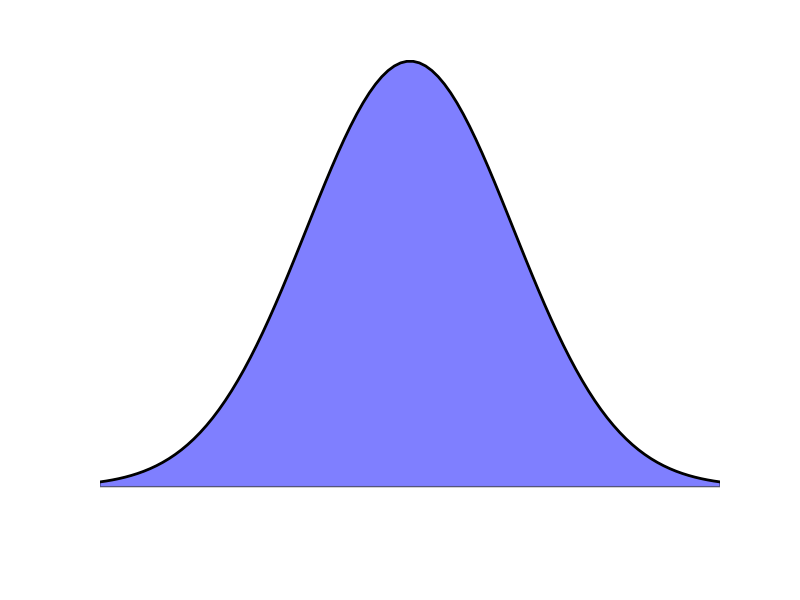
\includegraphics[width=.05\textwidth]{gaussian.png}};

    % First rectangle
    \draw (5,0) rectangle (8.5,3);
    \draw [fill=blue]   (5.5,1) rectangle (6,2);
    \draw [fill=green] (6.5,1) rectangle (7,2);
    \draw [fill=red]     (7.5,1) rectangle (8,2);

    % First gaussian filter
    \draw (1,6) rectangle (4.5,9);
    \draw (5,6) rectangle (8.5,9);
    \draw (9,6) rectangle (12.5,9);

    \draw [->,blue] (1.75,6) -- (2,5);
    \draw [->,blue] (2.75,6) -- (2.75,5.35);
    \draw [->,blue] (3.75,6) -- (3.5,5);
    \draw [->,blue] (2.75,4.5) -- (5,3);

    \draw [->,red] (9.75,6) -- (10,5);
    \draw [->,red] (10.75,6) -- (10.75,5.35);
    \draw [->,red] (11.75,6) -- (11.5,5);
    \draw [->,red] (10.75,4.5) -- (8.5,3);

    \draw [->,green] (5.75,6) -- (6,5);
    \draw [->,green] (6.75,6) -- (6.75,5.35);
    \draw [->,green] (7.75,6) -- (7.5,5);
    \draw [->,green] (6.75,4.5) -- (6.75,3);


    % middle rectangles 
    \draw (1,12) rectangle (4.5,15);
    \draw (5,12) rectangle (8.5,15);
    \draw (9,12) rectangle (12.5,15);

    \draw [fill=blue]   (1.5,13) rectangle (2,14);
    \draw [fill=blue]   (2.5,13) rectangle (3,14);
    \draw [fill=blue]   (3.5,13) rectangle (4,14);

    \draw [fill=green]   (5.5,13) rectangle (6,14);
    \draw [fill=green]   (6.5,13) rectangle (7,14);
    \draw [fill=green]   (7.5,13) rectangle (8,14);

    \draw [fill=red]   (9.5,13) rectangle (10,14);
    \draw [fill=red]   (10.5,13) rectangle (11,14);
    \draw [fill=red]   (11.5,13) rectangle (12,14);

    % small filter rectangles
    \draw (1,17) rectangle (2,18);
    \draw (2,17) rectangle (3,18);
    \draw (3,17) rectangle (4,18);

    \draw (5,17) rectangle (6,18);
    \draw (6,17) rectangle (7,18);
    \draw (7,17) rectangle (8,18);

    \draw (9,17) rectangle (10,18);
    \draw (10,17) rectangle (11,18);
    \draw (11,17) rectangle (12,18);

    % mult. rectangles and nodes
    \node at ( 2.75,10.5) [place] {$(*)$};
    \node at ( 6.75,10.5) [place] {$(*)$};
    \node at ( 10.75,10.5) [place] {$(*)$};

    \node at ( 2.75,19.5) [place] {$(*)$};
    \node at ( 6.75,19.5) [place] {$(*)$};
    \node at ( 10.75,19.5) [place] {$(*)$};

    % arrows of multiple rectangle nodes
    \draw [->,blue] (1.5,17) -- (1.5,15);
    \draw [->,blue] (5.5,17) -- (2.75,15);
    \draw [->,blue] (9.5,17) -- (3.75,15);

    \draw [->,green] (2.5,17) -- (5.5,15);
    \draw [->,green] (6.5,17) -- (6.75,15);
    \draw [->,green] (10.5,17) -- (7.75,15);

    \draw [->,red] (3.5,17) -- (9.5,15);
    \draw [->,red] (7.5,17) -- (10.75,15);
    \draw [->,red] (11.5,17) -- (11.75,15);

    % rectangles
    \draw (1,21) rectangle (4.5,24);
    \draw (5,21) rectangle (8.5,24);
    \draw (9,21) rectangle (12.5,24);

    \draw [fill=blue]   (1.5,22) rectangle (2,23);
    \draw [fill=green]   (2.5,22) rectangle (3,23);
    \draw [fill=red]   (3.5,22) rectangle (4,23);

    \draw [fill=blue]   (5.5,22) rectangle (6,23);
    \draw [fill=green]   (6.5,22) rectangle (7,23);
    \draw [fill=red]   (7.5,22) rectangle (8,23);

    \draw [fill=blue]   (9.5,22) rectangle (10,23);
    \draw [fill=green]   (10.5,22) rectangle (11,23);
    \draw [fill=red]   (11.5,22) rectangle (12,23);


    % sum nodes
    \node at ( 2.75,4.5) [place] {$\sum$};
    \node at ( 6.75,4.5) [place] {$\sum$};
    \node at ( 10.75,4.5) [place] {$\sum$};


\end{tikzpicture}
\end{document}
}
\fbox{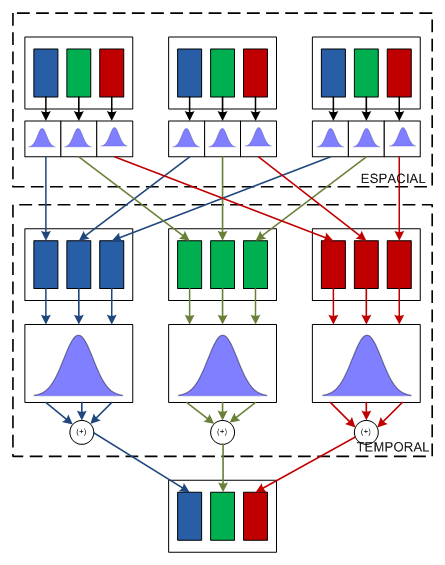
\includegraphics[scale=0.5]{img/Spatio_Temporal_Filter}}
\caption[Filtro temporal spacial]{Diagrama en bloques del filtro temporal y espacial. La parte de filtro temporal toma tres imágenes y aplica un filtro Gaussiano, el filtro espacial junta los componentes y aplica otro kernel Gaussiano.}
\label{fig:spatio_temporal_filter}
\end{figure}


Una representación en bloques de la implementación de este filtro se puede notar en la figura \ref{fig:spatio_temporal_filter}. La primera etapa es el procesamiento espacial, en que aplica un proceso de difuminado (\textit{blurring}) a cada uno de los colores de una imagen. Este procedimiento, es un suavizado Gaussiano que permite reducir el ruido en la imagen de cada uno de los componentes. La segunda etapa, consiste en agrupar por colores el resultado del filtrado espacial, para luego utilizar un segundo filtro Gaussiano, en cada uno de los tres componentes de las imágenes agrupadas por colores. El resultado es una suma de los tras componentes previamente filtrado. Finalmente, cada uno de los componentes se vuelven a juntar en una sola imagen con tres colores filtrados temporalmente.


La efectividad de este filtro puede ser comparado en los gráficos de la figura \ref{fig:result_spatio_temporal_filter}. La imagen \ref{fig:Figure_A} es el cluster de la imagen de fondo en funcionamiento normal del algoritmo sin filtro aplicado sobre las imágenes. En cambio la imagen de la figura \ref{fig:Figure_B} es el resultado final del cluster de la imagen de fondo,  aplicando procesamiento previo a las imágenes antes de ingresar en el algoritmo. Se puede observar que el cluster final filtrado es mucho más compacto que el otro. Finalmente esta de filtrado es una ayuda en el proceso de separación del fondo de imagen de los elementos móviles.

\begin{figure}
\centering     %%% not \center
\subfigure[Resultado final sin filtro]{\label{fig:Figure_A}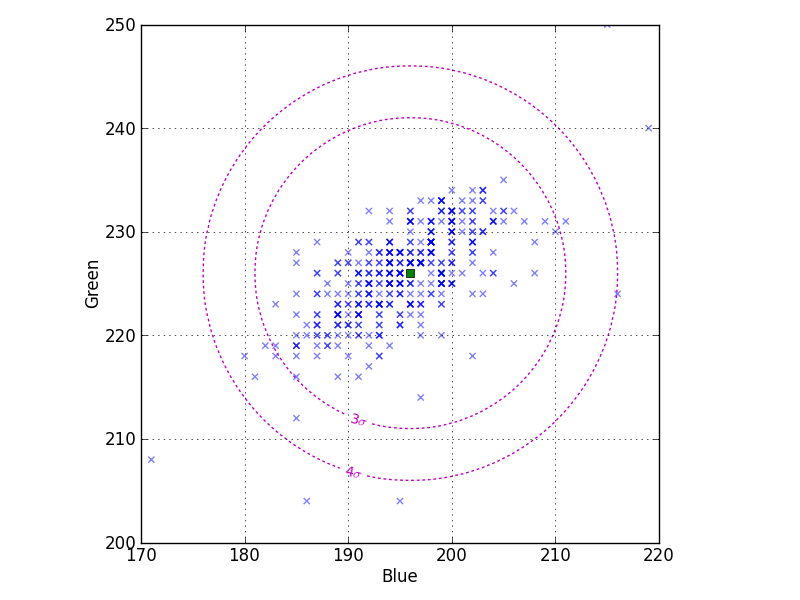
\includegraphics[width=70mm]{img/cluster_bg_340_160}}
\subfigure[Resultado final con filtro]{\label{fig:Figure_B}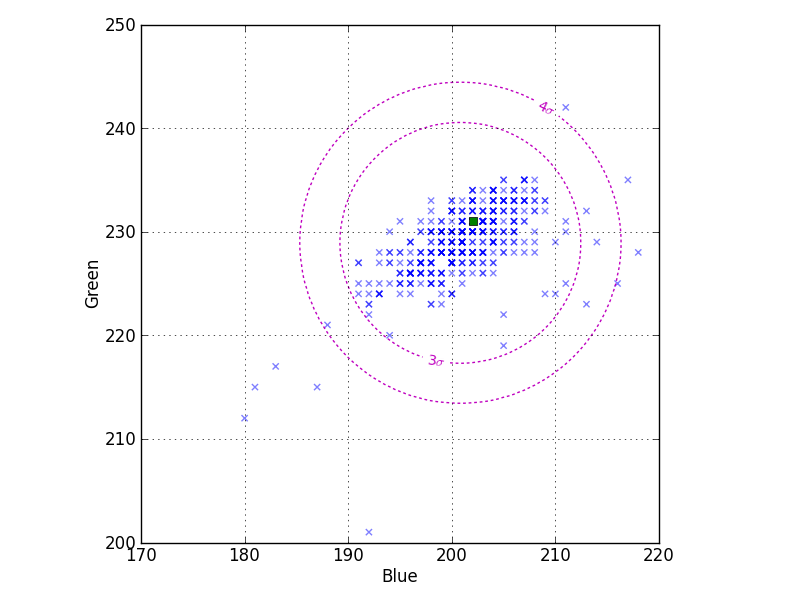
\includegraphics[width=70mm]{img/cluster_bg_340_160_filter}}
\caption[Comparación de efectividad del filtro en una secuencia completa]{Comparación de efectividad del filtro Espacial-Temporal aplicado en la secuencia completa }
\label{fig:result_spatio_temporal_filter}
\end{figure}




\chapter{Métricas de evaluación de rendimiento}\label{chap:metricas}
 
\section{Introducción}

Se encuentra en la literatura un conjunto heterogéneo de métodos de evaluación, que sirven para valorar la calidad de segmentación de un algoritmo. Pero, no existe acuerdo entre los investigadores para usar una metodología de evaluación general, que pueda proporcionar un criterio de comparación común, de medición del desempeño de los algoritmos de separación entre \emph{Foreground} y \emph{Background}. Asimismo, se han puesto a disposición de la comunidad una gran cantidad de escenarios de evaluación ("\emph{datasets}"), entre estos \cite{singh_muhavi_2010}, que establecen una serie de condiciones (ambientales, iluminación, etc) bajo las cuales, los algoritmos pueden experimentar diversas situaciones que les permitiría contrastar y evaluar su comportamiento en diferentes situaciones.

Estos métodos han sido clasificados en la literatura y dependiendo de la naturaleza del evaluador, en diversas metodologías que establecen dos categorías principales; \emph{método de evaluación subjetiva} \cite{mckoen_evaluation_2000} y \emph{método de evaluación objetiva}. Este capítulo presenta una descripción de los variados enfoques y métricas empleados en la actualidad para hacer evaluación de calidad, centrando el análisis en el criterio denominado evaluación objetiva.

\section{Enfoques de evaluación}

Las metodologías de evaluación \emph{subjetivas}, se basan en la valoración que hace un grupo de observadores, al resultado final de un proceso de segmentación. No obstante, requiere un gran número de evaluaciones, para producir un resultado con relevancia estadística. En contraste con el método anterior, las metodologías denominadas \emph{objetivas}, buscan una forma de evaluación automática que no requiera la intervención humana en el proceso de medición. En general, el resultado final es una mixtura de métricas, que elaboran un ranking de la calidad de segmentación en una imagen o secuencia de vídeo. Igualmente, el tipo de métricas empleadas en la evaluación objetiva, se dividen en métricas \emph{analíticas} y \emph{empíricas}. Las métricas analíticas requieren conocimiento del algoritmo, para evaluar sus requerimientos,  complejidad,  y estructura. Las métricas del tipo empíricas en cambio, miden calidad del resultado final de un proceso de segmentación.

Los métodos de evaluación del tipo empíricos se dividen a su vez, en métodos de \emph{discrepancia empírica} o \emph{evaluación relativa}, y métodos de \emph{evaluación autónomos}. Los métodos de discrepancia, se basan en medición de disparidad entre una imagen con anotaciones manuales o de referencia, ``ground truth'', y el resultado de segmentación. Las imágenes con anotaciones manuales funcionan como base de comparación, son mascaras binarias que etiqueta un pixel como background o foreground y tienen la finalidad de proporcionar un conjunto de datos independiente y objetivo, con el cual un resultado obtenido puede ser comparado y medido. Pero, estas mascaras son construidas manualmente, por lo que tienen en forma inherente un cierto grado de error e incertidumbre, que influye en la clasificación final como el mejor resultado que puede ser obtenido. Los métodos autónomos, en cambio, son métodos del tipo \emph{no-supervisados} \cite{zhang_image_2008} donde no requieren una imagen de referencia, evalúan el grado de igualdad de un conjunto de características de imágenes segmentadas previamente determinadas por evaluadores humanos.

Los métodos de evaluación más empleados son los basados en discrepancia empírica, los diferentes modelos propuestos en la literatura plantean una medición objetiva tratando de representar la percepción humana. Las distintas aproximaciones hacen una ponderación del resultado final de acuerdo con la visibilidad de los errores.



\section{Métodos de evaluación de calidad}

Esta parte se enfoca principalmente en métodos de evaluación de calidad basados en \emph{discrepancia empírica}, métodos que hacen una evaluación de percepción de los resultados. En los siguientes párrafos se hace una descripción y análisis de las métricas más recurrentes encontradas en la literatura para hacer evaluación de clasificación de objetos. 

\subsection{Error Cuadrático Medio y Relación a Señal Ruido}

Una de las formas más simples de medir calidad es el \emph{error cuadrático medio} (Median Squared Error - MSE) y la \emph{relación señal a ruido} (Peak Signal-to-Noise - PSNR) \cite{furht_handbook_2003} \cite{park_benchmark_2013}, el cual hace un promedio de el cuadrado de las diferencias de intensidad entre los pixeles de la imagen obtenida y su par de referencia, \emph{ground-truh}. A pesar, que es un método simple de calcular y promediar, ambas mediciones no tienen buena correlación con las medidas de percepción humana. En \cite{signal_zhou_2009} se demuestra mediante ejemplos, que \emph{MSE} no es una buen indicador para medir la fidelidad y calidad de una imagen. Se constatan valores similares de MSE en varias imágenes distorsionadas artificialmente (con respecto a una imagen original), no obstante las imágenes presentan calidades visuales muy diferentes.  También se hace notar en imágenes con pequeñas modificaciones geométricas, imperceptibles desde el punto de la calidad de percepción, valores de MSE muy grandes.

\begin{equation}
MSE=\frac{1}{N}\sum_{i=1}^N(x_{i}-y_{i})^2
\end{equation}

\begin{equation}
PSNR = 10\log_{10} {\frac{L^2}{MSE}}
\end{equation}

Donde $N$ es el número de pixeles de la imagen, $x_{i}$ e $y_{i}$ es el pixel $i$ de la imagen de referencia y resultante, respectivamente, y $L$ es el rango dinámico del valor de los pixeles. Para 8 bits este valor es 255.
 

\subsection{Métricas de Calidad Estática}

Estas métricas de calidad, son elaboradas realizando la comparación individual de un pixel de la imagen resultante, con el pixel equivalente de su imagen de referencia o \emph{ground-truth}. Es un procedimiento de comparación pixel-pixel, que entrega como resultado una serie de mediciones base, usadas posteriormente para construir estas métricas de calidad. La imagen de la figura \ref{fig:mask} es la mascara de una silueta después de haber sido separada de su imagen de fondo. Esta mascara señala en diferentes colores los resultados de comparación con su imagen de referencia (figura \ref{fig:gt}). El número $TP$ (\emph{verdaderos positivo}) de esta imagen, corresponde a los píxeles de la silueta (\emph{foreground}) correctamente clasificados. $TN$ (\emph{verdadero negativo}) es el número de píxeles de la imagen de fondo (\emph{background}) seleccionados correctamente. $FP$ (\emph{falso positivo}) es el número de pixeles pertenecientes a la imagen de fondo seleccionados incorrectamente como píxeles perteneciente a la silueta. $FN$ (\emph{falso negativo}) corresponde a un número de pixeles de la silueta incorrectamente clasificados como imagen de fondo. El resultado de estas mediciones se colocan en una matriz de confusión (conocida también como tabla de contingencia) para formar la base de todas métricas de evaluación de calidad, como se indica en figura \ref{fig:confusion_matrix}. 

\begin{figure}
\centering     %%% not \center
\subfigure[Mascara estimada]{\label{fig:mask}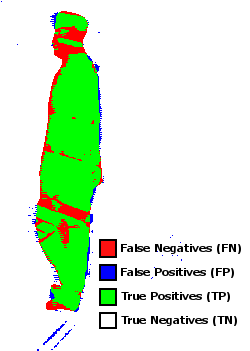
\includegraphics[width=50mm]{img/ch4/mask}}
\subfigure[Imagen de referencia]{\label{fig:gt}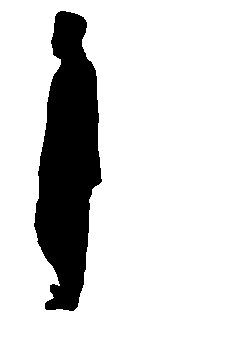
\includegraphics[width=50mm]{img/ch4/gt}}
\label{fig:metricas_calidad_estatica}
\caption[Métricas de calidad estática]{Métricas de calidad estática, imagen de referencia y mascara estimada por algoritmo}
\end{figure}

Una condición positiva de la imagen de referencia en esta tabla, se refiere a todos los píxeles que circunscriben la silueta (\emph{foreground}) que un algoritmo debiera separar del fondo de imagen, y la condición negativa son todos los píxeles que están en el fondo de la imagen. En otro aspecto, la condición positiva en el resultado de la separación (mascara) son todos los píxeles que fueron clasificados pertenecientes a la silueta, y la condición negativa son todos los píxeles clasificados en la imagen de fondo. Los números localizados en la diagonal principal de esta matriz representan decisión correcta ($TP$ y $TN$) y los números de diagonal opuesta ($FN$ y $FP$) son los errores (``confusión'') realizados durante la clasificación, en este caso son los errores del algoritmo al equivocar píxeles de la imagen de fondo con píxeles de la silueta y píxeles de una silueta con los de la imagen de fondo.




\[
Precision=\frac{Total \: pixeles \, en \, foreground \, clasificados \, correctamente}{Total \, pixeles \, imagen \, resultante}
\]\\
\[
Recall=\frac{Total \: pixeles \: foreground \, clasificados \, correctamente}{Total \, foreground \, pixeles \, de \, imagen \, referencia}
\]\\
\[
True Positive Rate=\frac{Positivos  \: (silueta) \: clasificados \, correctamente}{Total \, positivos}
\]\\
\[
False Negative Rate=\frac{Negatives  \: (background) \: clasificados \, incorrectamente}{Total \, negativos}
\]


\begin{figure}[!ht]
\centering
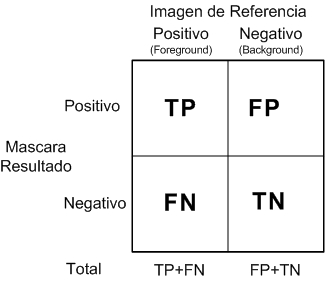
\includegraphics[scale=0.6]{img/ch4/Confusion_Matrix}
\caption{Matriz de Confusión}
\label{fig:confusion_matrix}
\end{figure}



A partir de esta matriz de contingencia, se determinan una serie de métricas comunes de calidad, que se utilizan en los algoritmos de clasificación. La \textbf{tasa verdaderos positivos} (\textit{true positive rate}) es una medida de proporción de los positivos (píxeles de la silueta) seleccionados correctamente, está métrica también es conocida como \textit{recall} o \textit{sensitivity}. La \textbf{tasa falsos positivos} (\textit{false positive rate}) o tasa de falsas alarmas, corresponden a la proporción de negativos (píxeles \textit{background}) clasificados incorrectamente. Una medida complementaria a la tasa de falsos positivos es la métrica de \textit{specificity}, el cual es una proporción de negativos (\textit{background}) clasificados correctamente. En sistemas de recuperación de información (\emph{Information Retrieval}) las medidas de \emph{precision} (proporción de píxeles seleccionados correctamente), \emph{recall} y media armónica \emph{F-Measure} \cite{brutzer_evaluation_2011} \cite{herrero_background_2009} \cite{park_benchmark_2013} (medida de desempeño total) son muy utilizadas como métricas de evaluación de rendimiento, está medición esta entre el rango $0, 1$. En el caso de separación de foreground y background, un valor alto de \emph{F-measure} es un indicador para una mejor segmentación del foreground.



\begin{equation} \label{eq:precision}
Precision = \frac{TP}{TP + FP}
\end{equation}
\begin{equation} \label{eq:tpr}
True \: Positive \; Rate = \frac{TP}{TP+FN}
\end{equation}
\begin{equation} \label{eq:fpr}
False \; Positive \; Rate = \frac{FP}{FP + TN}
\end{equation}\\
\[
sensitivity = recall 
\]
\[
specificity = 1 - fpr
\]\\
\begin{equation} \label{eq:fmeasure}
F-Measure = \frac{1}{\frac{1}{precision} + \frac{1}{recall}}
\end{equation}

Las mediciones de la matriz de confusión se pueden relacionar también, con un indicador de correlación denominado \emph{Matthew Correlation Coefficient - MCC}. Ésta es una medida de calidad de clasificación de dos clases diferentes. Es un coeficiente de correlación entre la referencia y el resultado obtenido (observado). El rango de valores para este coeficiente, varía entre $-1, 1$ ($MCC \in [-1,1]$). Un resultado con valor $1$ indica un resultado perfecto, el $0$ representa un valor no mejor que un resultado aleatorio, y $-1$ es una total diferencia entre los obtenido y la referencia.

\begin{equation} \label{eq:mcc}
MCC = \frac{TP X TN - FP X FN}{\sqrt[2]{(TP + FP)(TP + FN)(TN + FP)(TN + FN)}}
\end{equation}


\subsection{Curva de operaciones característica}
\label{subsec:roc}
Los algoritmos de sustracción de imágenes de fondo o separación de \emph{foreground} y \emph{background}, son métodos que clasifican un píxel perteneciente a la imagen de fondo o a un objeto que está en movimiento, como una silueta del actor (\emph{foreground}). La curva de operaciones características (\textit{receiver operating characteristics - ROC}) es un gráfico que permite visualizar en forma global el desempeño de clasificación de un algoritmo. Un punto en esta curva relaciona la respuesta de clasificación, en este caso proporción de píxeles clasificados correctamente, con la proporción de píxeles negativos incorrectos. Describe un balance relativo entre beneficios (\emph{verdaderos positivos}) y costos (\emph{falsos positivos}). La curva se construye con el resultado de varias operaciones distintas, utilizando el mismo conjunto de datos, pero modificando algún parámetro característico de este algoritmo. Esto permite comparar el desempeño con diferentes configuraciones de un algoritmo.

La figura \ref{fig:tpr_fpr} es una curva ROC de ejemplo, que muestra el resultado de dos algoritmos diferentes. El punto (0,0) de la esquina inferior izquierda representa una estrategia de nunca producir una clasificación positiva, un algoritmo localizado en este punto no genera errores de falso positivo, pero tampoco obtiene verdadero positivos. El punto (1,1) es opuesto al anterior, siempre tiene clasificaciones positivas. El punto (0,1) es el resultado de clasificación perfecta, los píxeles en foreground fueron detectados completamente, sin errores en los píxeles de la imagen de fondo. Un punto en el espacio ROC es mejor que otro, sí esta localizado más cerca de la esquina superior izquierda que el otro punto; el algoritmo presenta una tasa de verdaderos positivos alta y una tasa de falsos positivos baja. Algoritmos que se ubican en la parte izquierda del gráfico, cercano al eje X, se pueden considerar ``convervadores'', hacen una clasificación positiva teniendo buena evidencia, tienen muy poco errores de falso positivo, pero tienen también una baja tasa de verdaderos positivos. Al contrario, algoritmos que se ubican en la parte superior derecha de la gráfica, son algoritmos más libres, hacen clasificaciones positivas con poca evidencia, clasificando todos los positivos correctamente, pero con una alta tasa de falsos positivos. 

La recta $y=x$ representa una estrategia de estimación aleatoria, en algoritmos de clasificación binaria. Cualquier punto en esta recta, implica el mismo valor de clasificación para ambas clases. Por ejemplo, un algoritmo que hace una estimación aleatoria de obtener una silueta la mitad del tiempo, se puede esperar que obtenga la mitad de silueta y el fondo de imagen en forma correcta, ubicando esta clasificación en el punto (0.5, 0.5) de la gráfica ROC. Sí se estima por ejemplo que la estimación de la silueta es positiva el 90\% del tiempo, se puede esperar conseguir un 90\% de tasa de verdaderos positivos, pero con un incremento de la tasa de falsos negativos a un 90\% también.




\begin{figure}[!ht]
\centering
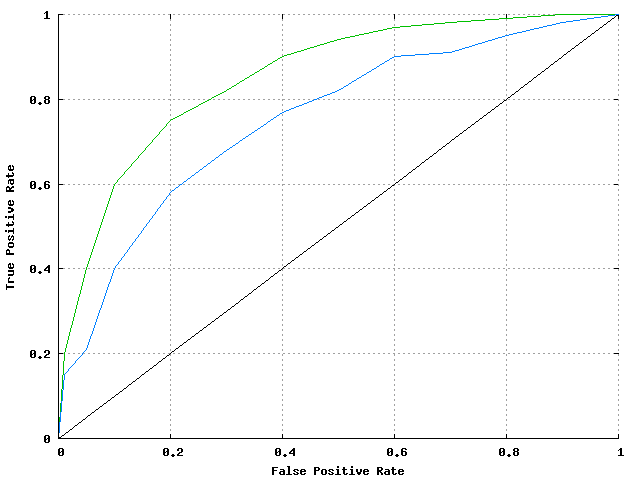
\includegraphics[scale=0.5]{img/ch4/curva_operaciones_caracteristicas}
\caption{Curva de operaciones características}
\label{fig:tpr_fpr}
\end{figure}




\subsection{Métricas de Percepción}
\label{sub:metricas_percepcion}

Estas métricas intentan ponderar el concepto de percepción de un observador, sobre el resultado final de segmentación. Se propone cuantificar los conceptos de \emph{exactitud espacial} (spatial accuracy) y \emph{estabilidad temporal} \cite{liu_metrics_2011} \cite{cavallaro_objective_2002} o \emph{coherencia temporal} \cite{villegas_perceptually-weighted_2004}. Ponderan, mediante algún tipo de función definida, la discrepancia entre una mascara estimada y la de su referencia (ground-truth), tomando en cuenta la inexactitud potencial que puede contener la mascara de referencia, la localización de los pixeles con errores relativo al borde de la mascara de referencia, y el tipo de errores (FP, FN). 

\subsubsection{Contexto espacial y temporal}
El contexto espacial \cite{cavallaro_objective_2002} de un pixel errado, es caracterizado por la distancia más cercana de un objeto detectado. Esta propiedad relaciona el foco de atención de un observador hacia a un objeto que le llama la atención, errores del tipo falso negativo (pixel clasificado erróneamente como foreground) son más importantes en la medida que la distancia es mayor. El contexto temporal considera las diferencias de calidad en el tiempo, para esto identifican dos tipos de fenómenos; un efecto sorpresa y un efecto fatiga. El efecto sorpresa se relaciona con los cambios en la exactitud espacial y el efecto fatiga se relaciona con el hecho de un observador se acostumbra a cierto tipo de calidad en el tiempo. Estos dos contextos son relacionados en las siguientes expresiones.

\begin{equation}
\nu_w(n) = 1 - \epsilon_w(n)
\end{equation}

\begin{equation}
\zeta_w(n) = \frac{\nu_w(n)}{2} \lbrack 1 + \alpha_t \frac{d}{dn}\nu(n) \rbrack
\end{equation}

Siendo $\nu_w(n)$ un valor de ponderación de la exactitud espacial, $\frac{d}{dn}\nu(n)$ variación espacial en el tiempo (mientras mayor esta variación más pequeño su coherencia temporal) y $\zeta_w(n)$ una medida de calidad de percepción espacial-temporal. Se define una \emph{exactitud espacial absoluta} y \emph{relativa} (normalización por el total de pixeles) como la contribución de las ponderaciones de $w^i_p$ (falso positivo), y $w^j_n$ (falso negativo) . 

\begin{equation}
w^i_p = \frac{\alpha_p \log(d^i_p + 1)}{D}
\end{equation}

\begin{equation}
w^i_j = \frac{\alpha_nd^j_n}{D}
\end{equation}

\begin{equation}
\epsilon_w() = \sum_{i=1}^{\epsilon_p(n)}w^i_p +	 \sum_{j=1}^{\epsilon_n(n)} w^j_n
\end{equation}


\begin{figure}[!ht]
\centering
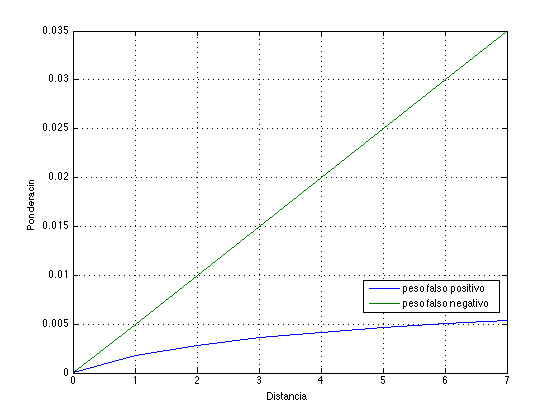
\includegraphics[scale=0.4]{img/ch4/PesosFalsoPositivoNegativo}
\caption{Pesos pixeles falso positivo y negativo}
\label{fig:Contexto espacial pesos para pixeles falso positivo y negativo}
\end{figure}

Como se indica en la figura 2, ambas ponderaciones o pesos $w^i_p$ y $w^j_n$ aumentan con la distancia, pero influyen en forma diferenciada en la ponderación final de exactitud espacial. Los pesos para falsos positivos se incrementan en forma lineal, y estos valores son mayores con los pesos de los falsos negativos a la misma distancia.

\subsubsection{Observaciones para cuantificación espacial}

Las mediciones de exactitud espacial del trabajo propuesto en \cite{liu_metrics_2011}, se basan en observaciones que toman en consideración, el error producido al generar las mascaras de referencia en forma manual. Se menciona que los pixeles errados, muy cerca de los bordes de las mascaras de referencia, se presumen causados por la inexactitud durante la creación de estas mascaras. A su vez, una segunda observación indica que estos mismos errores muy cercanos al borde, tienen poco efecto comparado con otro que se encuentra muy lejano del borde. Pese a que estos pixeles en el borde hacen que un objeto parezca más grueso o delgado, estos no cambian la forma del objeto. Una tercera observación, señala que el impacto de los diferentes tipos de errores durante el procesamiento no son similares, por lo que hacen las distinción de medir en forma independiente falsos negativos y falsos positivos. 

Se propone una función ponderación del tipo sigmoidal, de esta forma errores muy cercanos al borde de la mascara tienen un valor (peso) menor a uno y otros errores lejanos al borde se aproximan a uno. 

\begin{equation}
S(d;\alpha) = \frac{1 - e^{-\alpha \cdot d}}{1 + e^{-\alpha \cdot d}}
\end{equation}

Esta función $S$, tiene como variable $d$ distancia de un pixel en error al borde de la mascara, y $\alpha$ es parámetro que modela la tolerancia de la inexactitud de las mascaras de referencia en sus bordes. Un parámetro $\alpha$ pequeño conlleva una capacidad de tolerancia mayor. 

\begin{figure}[!ht]
\centering
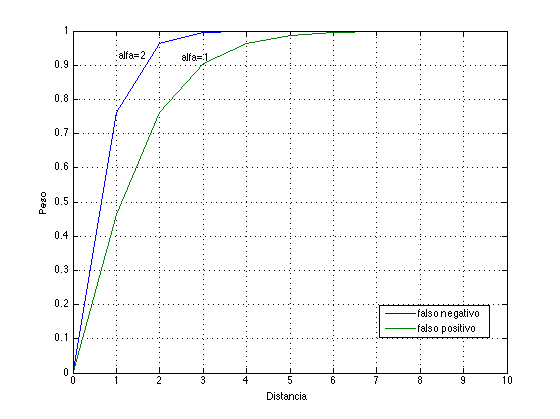
\includegraphics[scale=0.4]{img/ch4/sigmoid_function}
\caption{Pesos usando función tipo sigmoidal}
\label{fig:Pesos tipo sigmoidal}
\end{figure}


\subsection{Similaridad Estructural}
El índice de \emph{similaridad estructural} - \emph{SSIM} (\emph{Structural SIMilarity}) \cite{park_benchmark_2013} \cite{wang_image_2004} es un método de medición de similaridad entre dos imágenes. Es una medida de calidad de una imagen de entrada contrastada con otra de buena calidad. Este índice usa un nuevo enfoque para medir calidad, se basa en la hipótesis que la principal función del ojo humano  es extraer información estructural de su campo visual, y además el Sistema Visual Humano (\emph{Human Visual System - HVS}) está muy adaptado para realizar esta operación. Por lo tanto una medición de distorsión estructural podría ser una buena aproximación. Se platean entonces, en este nuevo enfoque, moverse desde mediciones de errores (métodos vistos anteriormente) a realizar mediciones de distorsión estructural. Sin embargo, el nuevo problema que se debe enfrentar es cómo definir y cuantificar distorsiones estructurales.

El modo de medir y obtener el índice \emph{SSIM} supone una secuencia de imágenes de entrada en escala de grises además de la secuencia de imágenes de referencia, ground-truth. Se considera la secuencia de referencia como la secuencia con las imágenes de buena calidad, de esta forma la medida de similaridad sirve como una medición de la calidad de la otra secuencia de entrada. La manera de medir similaridad es separar la tarea en tres componentes; \emph{luminancia}, \emph{contraste}, y \emph{estructura}.

\begin{equation}
SSIM(x,y) = f(l(x,y), c(x,y),s(x,y)) 
\end{equation}

\begin{equation}
SSIM(S,G) = (\frac{2\mu_S\mu_G + c_1}{\mu_S^2 + \mu_G^2 + c_1}) \cdot (\frac{2\sigma_S\sigma_G + c_2}{\sigma_S^2\sigma_G^2 + c_2}) \cdot (\frac{\mu_{SG} + c_3}{\mu_S\mu_G + c_3})
\end{equation}

Este índice de calidad es una combinación de tres factores, pérdida de correlación, distorsión media, y varianza de la distorsión. El primer componente es el coeficiente de correlación lineal entre $S$ y $G$ y su rango dinámico varia en $[-1,1]$. El segundo componente mide similaridad entre valores medios, y su rango de valores está entre $[0,1]$. El tercer componente mide similaridad entre las varianzas de ambas imágenes de una secuencia, y su rango dinámico está entre $[0,1]$. La relación final aplicada sobre secuencia de vídeo viene dada por la siguiente formula. 


\begin{equation}
SSIM(S,G) = \frac{1}{n} \sum_{i=1}^{n} \frac{(2\mu_{S_{i}} \mu_{G_{i}} + c_1) \cdot (2 cov_{S_iG_i} + c_2)}  {(\mu^2_{S_i} + \mu^2_{G_i} + c_1) \cdot (\sigma^2_{S_i} + \sigma^2_{G_i} + c_2)}
\end{equation}

Donde, $S$ es un conjunto de $n$ imágenes resultantes, $G$ conjunto de las imágenes de referencia (ground-truth), $\mu_{S_i}$ $\mu_{G_i}$ media de ambas secuencias, $\sigma_{S_i}$ y $\sigma_{G_i}$ desviaciones estándar, y $cov_{S_iG_i}$ covarianza de $S_i$ y $G_i$. Las constantes $c_1 = (k_1 + L)^2$ $c_2=(k_2 + L)^2$ con valores $k_1=0.01$ $k_2=0.03$ y $L=255$.


\subsection{D-Score}
D-Score brinda un criterio de \emph{disimilitud} entre una imagen de referencia y la imagen de entrada, esta métrica sólo considera fallas en la medición de los resultados. El costo de un error depende de la distancia con el objeto más cercano de la referencia, teniendo una ponderación mayor los errores en el rango intermedio. Esto debido que este tipo de errores impactan de mayor manera el reconocimiento de formas. Por ende, errores en zonas lejanas/cercanas tendran un D-score cercano a cero. 

\begin{equation}
DT(x) = min( d(p,x), \forall x \in X)
\end{equation}

El costo de error se basa en una \emph{Tranformada de Distancia} (Distant Transform - DT) de la referencia ground-truth, con $X$ un conjunto de pixeles de referencia, $d(p,x)$ es la distancia del pixel $p$ al pixel $x$, entonces $DT(x)$ es la distancia mínima entre un pixel $x$ y el punto de referencia más cercano. Para calcular $DT(x)$ se usa la siguiente relación

\begin{equation}
D-score(x) = exp( - (\log_2(2.DT(x)) - \alpha )^2)
\end{equation}


\begin{figure}[!ht]
\centering
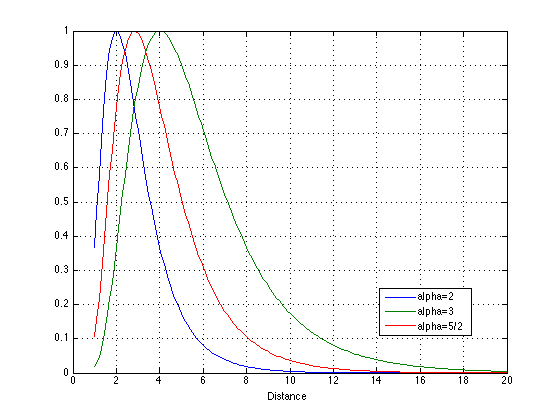
\includegraphics[scale=0.4]{img/ch4/dscore}
\caption{Valores D-Score basados en la distancia desde la referencia ground-truth}
\label{fig:Valores D-Score}
\end{figure}

De acuerdo con la figura 4, se tiene una tolerancia de 3 pixeles desde la referencia, esto debido que ese tipo de errores locales no afecta realmente el proceso de reconocimiento. De esta misma forma tomando un valor de $\alpha=5/2$, \cite{park_benchmark_2013}, se permiten que ocurran errores a más de 10 pixeles de distancia. D-score entrega un índice que señala el nivel de reconocimiento de objetos, en la medida que este valor es menor, mejor es el reconomiciento, independiente del valor de errores que entreguen otros índices, como el \emph{F-Measure}.

\section{Resumen de métodos de evaluación}
Se ha hecho una descripción de la mayoría de los métodos de medición utilizados actualmente, basados principalmente en el paradigma de evaluación por discrepancia  o error. Una menor discrepancia con una referencia, brindan un ranking de mayor calidad de clasificación o comparación de algoritmos. En general, no existe una métrica ideal, que pueda ser utilizada como herramienta de comparación universal, entre los diferentes algoritmos existentes. De igual modo, estas métricas pueden ser empleadas en conjunto, de manera complementaría, aprovechando las diferentes características de ellas. Un caso concreto es el trabajo desarrollado para el desafío BMC \cite{park_benchmark_2013}.

Las métricas más empleadas sin duda son ``\textit{Specificity}'' ($1-fp\; rate$), ``\textit{Sensitivity}'' (recall) y todas sus demás variantes, estas métricas proporcionan una medida general del resultado de clasificación. Presentan el compromiso entre la habilidad del algoritmo para identificar los píxeles correspondientes a una silueta (\emph{sensitivity}), y la habilidad del mismo algoritmo para identificar los píxeles pertenecientes a la imagen de fondo (\emph{specificity}). Estas dos métricas se colocan en una curva de ROC que permite comparar desempeño con otro algoritmo bajo las mismas condiciones. 

Las diferentes métodos basadas en el concepto de percepción se aproximan a una forma de evaluación que podría hacer un observador humano, para esto, hacen una combinación de un contexto espacial con un contexto temporal. Los errores se ponderan de acuerdo con distancia al borde de la mascara de referencia, la estabilidad de esta percepción espacial es además considerada en la evaluación de calidad. Los distintos enfoques encontrados de esta metodología se diferencian en el tipo de función empleada para hacer la ponderación espacial de los errores con respecto a la distancia del borde de su mascara. Evalúan con mayor ponderación el error falso negativo y localizado lejano al borde de la mascara. La métrica de ``D-Scorre'', a diferencia de la descripción previa castiga fuertemente los pixeles errados en el borde de la mascara, porque este tipo de errores no permiten realizar una buena clasificación.

Un diferente enfoque presenta el índice de similaridad, este ya no utiliza las mediciones de percepción para evaluar calidad. Postula medición de distorsión estructural, para esto se propone una combinación de mediciones de luminancia, contraste y estructura. Que vienen siendo análisis de correlación entre dos imágenes, cuantificación de sus varianzas y sus medias. 

Finalmente, estas distintas métricas pueden ser empleadas en conjunto o en forma individual. Pero una combinación de ellas podría brindar una mejor claridad desde el punto de vista de la calidad de los diferentes algoritmos. Pueden entregar una mejor discriminación de las ventajas y falencias en diversas condiciones ambientales. Se podría determinar un buen algoritmo para ciertas condiciones, pero también determinar sus desventajas en otras situaciones. 






\chapter{Herramientas de evaluación de algoritmos}

\section{Introducción}
La solución de software propuesta, es un conjunto de bibliotecas desarrolladas en lenguaje de programación C++ orientado a objetos. Este grupo de bibliotecas de clases posibilitan, por una parte, construir una simple aplicación cliente, que incorpora los algoritmos de visión de computador que se quieren verificar, y por otra parte, evaluar resultados logrados con el cliente proporcionado por este sistema (u otro independiente). Comparando posteriormente, el resultado con las imágenes de referencias, suministrada por el conjunto de datos que esta bajo evaluación. El software proporciona las interfaces necesarias, que simplifican la creación de instancias, de los algoritmos incluidos en el sistema de software. Facilita también, la incorporación de nuevos algoritmos, encapsulando las bibliotecas (de estos algoritmos) en una clase que contiene las operaciones predeterminadas, reconocidas por el sistema de software. 

Otro aspecto importante de esta solución de software, constituye la herramienta de evaluación de desempeño. Ésta fue proyectada, desde un principio, como un cliente que recibe de entrada un conjunto de imágenes procesadas, y otro conjunto de imágenes de referencia (\textit{ground-truth}). La salida es un resumen de desempeño, producto de la comparación de cada imagen. Este diseño, es independiente de la plataforma sobre el cual se ejecuta el algoritmo medido. La evaluación se realiza sobre las imágenes resultantes, previamente procesadas por los algoritmos que se intentan medir. Esta herramienta de software, incluye las métricas más comunes utilizadas en segmentación de imágenes, y un par de métricas relacionadas con la medición de percepción: similaridad estructural \cite{park_benchmark_2013, wang_image_2004}, y D-Score\cite{lallier_testing_2011}. El producto final es un archivo de texto, que contiene los resultados obtenidos para cada imagen y un valor acumulado total que informa el desempeño global del algoritmo logrado en toda la secuencia.


\begin{figure}[h!]
\centering
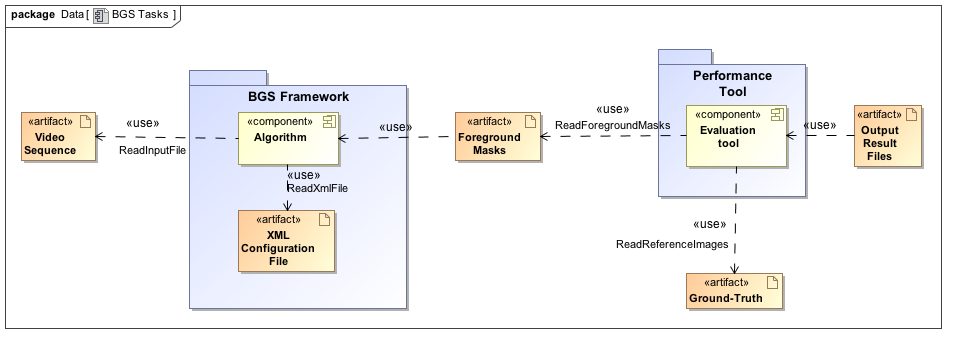
\includegraphics[scale=0.5]{img/BGS_Tasks}
\caption[Diagrama de componentes]{Diagrama de operación de los componentes de software.}
\label{fig:bgs_tasks}
\end{figure}



\section{Arquitectura de Software}

La arquitectura de software está basada en módulos. Cada módulo es una unidad independiente de software, basado en programación orientada a objetos. Facilita un conjunto de clases en C++, para ser utilizadas por los programas clientes, en los distinto niveles que ha sido estructurado de la arquitectura de este software. Los distintos módulos hacen uso de las bibliotecas de otros módulos para utilizar las facilidades que proporcionan cada uno de ellos.  

\begin{figure}[h!]
\centering
%\fbox{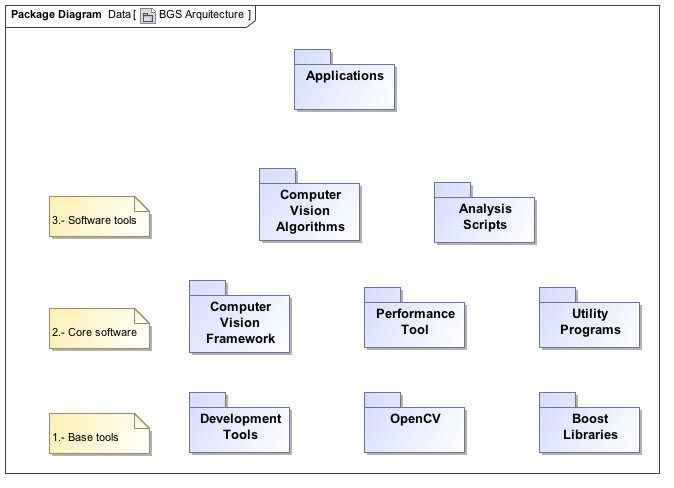
\includegraphics[scale=0.8]{img/BGS_Arquitecture}}
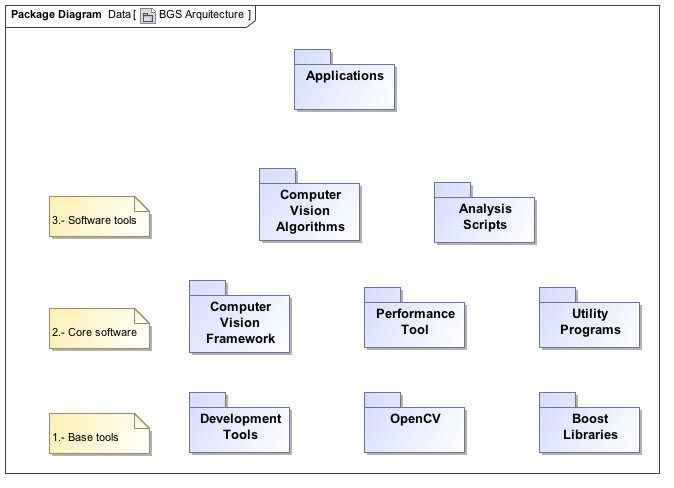
\includegraphics[scale=0.7]{img/BGS_Arquitecture}
\caption[Arquitectura modular de software]{Diagrama de la arquitectura de software propuesta.}
\label{fig:arq_software}
\end{figure}
 

\subsection{Herramientas Base}

La primera parte esta constituido principalmente, por las herramientas de desarrollo utilizados, como el compilador de C++, el repositorio de software donde se mantiene el control de versiones de los módulos. Las bibliotecas de OpenCV y Boost.

\subsubsection{Herramientas de desarrollo}
El desarrollo de los diferentes módulos de este software ha sido realizado en una distribución Linux, \textit{Ubuntu} 12.04 LTS precise. Ubuntu es un sistema operativo Linux, basado en Debian, que incluye todas las herramientas necesarias para hacer la implementación de los paquetes de software de esta solución. A continuación, se hace una breve descripción de los diferentes productos utilizados.

\begin{itemize}
\item \textbf{Compilador} GNU GCC versión 4.6
\item \textbf{CMake} es un grupo de herramientas, \textit{open source} independiente del sistema operativo, diseñado para construir, validar paquetes de software. Se ha usado principalmente para generar los archivos \textit{Makefile} nativos al sistema operativo Ubuntu. La utilidad de CMake, radica principalmente, en la independencia de la plataforma sobre la cual se está desarrollando. En caso de ser necesario, los módulos de software también pueden ser compilados y ejecutados en otros ambientes (MAC OS X, otros ``distros'' de Linux, o Windows).
\item \textbf{Servidor de repositorios \textit{GitHub}}, para llevar el control de cambios de versión de los distintos módulos. Este servicio de repositorio público, se basa en \textit{GIT} un sistema de control de versiones distribuidos. Las principales características, entre varias otras más, es un sistema de control de los datos, almacena el estado de un proyecto a nivel de directorios y archivos. Crea un registro completo (\textit{snapshot}) del repositorio que esta siendo almacenado, esto facilita las tareas de recuperación, creación de ramas de desarrollo (\textit{branch}) y unión (\textit{merge}) de diferentes versiones de un módulo. El proyecto completo puede ser localizado en el siguiente URL: \textit{https://github.com/jorgesep/BGS}. 
\end{itemize}


\subsubsection{Biblioteca OpenCV}
OpenCV \cite{opencv} (\textit{Open Source Computer Vision Library}) es una biblioteca que contiene una gran cantidad de algoritmos muy utilizados en visión por computador. La API (\textit{Application Programming Interface}) de OpenCV comprende una serie de módulos, que abarcan varios de los aspectos que se requieren para construir una aplicación en visión por computador. El módulo principal, define las estructuras básicas sobre la cual se desarrollan todas las aplicaciones, incluido los módulos de software construidos en este proyecto de tesis. Establece un arreglo, denominado \textit{Mat}, de varias dimensiones que permite contener en forma nativa,  la estructura de una imagen sobre la cual se pueden hacer todas las operaciones matriciales básicas, necesarias en visión por computador para manipular imágenes. Incluye también, un modulo de procesamiento de imágenes (filtros lineales y no-lineales, transformación geométrica de imágenes, conversión de espacio de colores, histogramas, entre otros). Un módulo de análisis de videos, que contiene varios algoritmos, entre ellos el algoritmo (\textit{Background Subtraction}) original de  \textit{Zivkovic y Heidjen} \cite{zivkovic_efficient_2006} evaluado en este trabajo.  Se agregan además, algoritmos de calibración, detectores de características, detección de objetos, una interfaz (\textit{gui}) para la captura de imágenes de video, \textit{codecs} de imágenes. También incluye un módulo para trabajar con GPU.


\begin{figure}[h!]
\centering
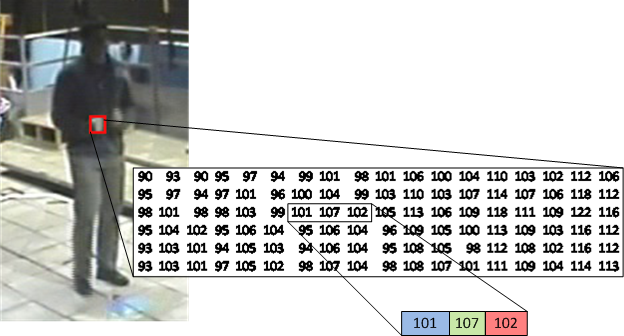
\includegraphics[scale=0.7]{img/Opencv_mat}
\caption[OpenCV arreglo Mat ]{Descripción del arreglo básico MAT de OpenCV}
\label{fig:mat}
\end{figure}


La estructura de datos \textit{Mat}, es una clase C++ de n-dimensiones, constituida en dos partes. Tiene un encabezado de la matriz de datos, que contiene información del tamaño de la matriz, el método utilizado para almacenar la matriz, la dirección de memoria donde se encuentra localizada la matriz de datos, entre otro tipo de información. Mantiene también, un puntero de la zona de memoria donde se encuentra la matriz de píxeles, y su dimensionalidad depende del método empleado para almacenar los datos. El encabezado de la matriz es constante, pero el tamaño de la matriz varia dependiendo del tipo de imagen que esta siendo manipulada. La figura \ref{fig:mat} es un ejemplo de esta matriz, la zona demarcada por el rectángulo en rojo es una zona de interés que se desea estudiar. La zona es una matriz de números manejada por la matriz \textit{Mat}, en el caso de una imagen definida en el espacio RGB, se almacenan los valores de cada píxel, en forma contigua, en el orden: blue, green, y red. Las líneas de códigos que se indican a continuación, es un ejemplo de la facilidad de uso de la estructura de datos \textit{Mat}.\\


\begin{lstlisting}
Mat A, C;                   // creates just the header parts
A = imread("File.jpg" , CV_LOAD_IMAGE_COLOR); // allocate matrix
Mat B(A);                   // Use the copy constructor
C = A;    
\end{lstlisting}

\subsubsection{Biblioteca Boost}
Boost \cite{boost} se ha usado principalmente para, evitar el problema que se encuentra al manipular archivos, operar con \textit{strings} de caracteres en C++. \textit{Boost} contiene varias bibliotecas utilitarias, y en este proyecto se han usado especialmente las que permiten manejar expresiones regulares, búsqueda de caracteres en una linea de \textit{strings}, reemplazo de caracteres, manipulación de archivos: $boost::filesystem$, $boost::system$, $boost::program_options$, $boost::reg_exp$.


\subsection{Descripción de sistemas de software}
La segunda parte de la implementación de este sistema, de acuerdo con el esquema de la figura \ref{fig:arq_software}, está compuesto por dos módulos principales e independientes. El módulo de \textit{Framework} que permite incorporar y verificar los diferentes algoritmos, y el módulo que incluye diferentes métricas de evaluación de desempeño. Como señala el diagrama de componentes (operación), la figura \ref{fig:bgs_tasks}, los módulos son independientes y funcionan en tiempos diferentes. La salida del primero, es la entrada del segundo.

\subsubsection{Framework de algoritmos}

La entrada de este \textit{framework} puede ser un archivo de video o  conjunto de imágenes secuenciales en cualquier formato (jpg, png, etc). Su salida son mascaras de siluetas (\textit{foreground}), generadas por el algoritmo seleccionado. Los resultados (mascaras) son almacenados en directorios independientes, (se crea un directorio por algoritmo configurado). De esta manera, se podrían ejecutar uno o más algoritmos en forma simultánea, dependiendo de un archivo \textit{xml} general de configuración. La configuración de cada uno de los algoritmos incluidos, también se realiza a través de archivos XML de configuración. Por cada algoritmo incluido en este \textit{framework} existe un archivo XML de configuración. Los archivos XML contienen parámetros necesarios que necesita el algoritmo para ser ajustado a los requerimientos de operación, entre estos se encuentran por ejemplo, la tasa de aprendizaje, valores por defecto de las distribuciones que modelan el fondo de imagen. 


\subsubsection{Diagrama de clases}
Se ha utilizado un patrón de diseño \cite{gamma_design_1995} \textbf{estrategia} (\textit{Strategy}) para implementar el \textit{framework} que da soporte a los distintos algoritmos.  Los patrones de diseño\cite{gamma_design_1995} son esencialmente un conjunto de soluciones a problemas repetitivos que se encuentran en el desarrollo de software. Utilizar un patrón de diseño es aprovechar la experiencia para enfrentar un problema conocido, re-usando una solución ya comprobada. 

\begin{figure}[h!]
\centering
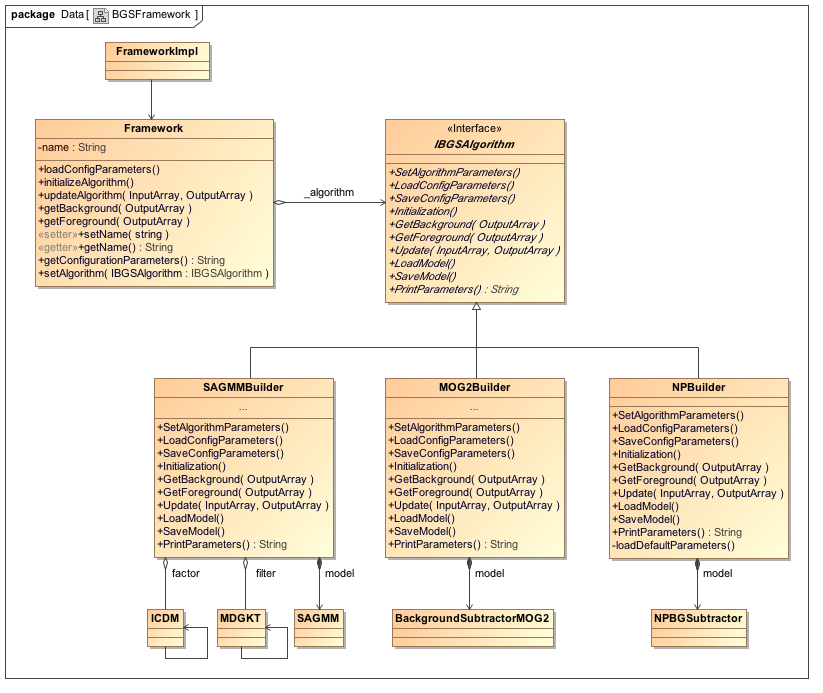
\includegraphics[scale=0.5]{img/BGSFramework}
\caption[Diagrama UML de clases Framework]{Diagrama UML de clases del framework de algoritmos}
\label{fig:uml_framework}
\end{figure}

El patrón de diseño estrategia, en este caso, se usa para encapsular los algoritmos y hacerlos intercambiables, al ser invocados por algún cliente en tiempo de ejecución. Se basa en la idea de encapsular el comportamiento de la parte que cambia. Aprovecha la propiedad de ``polimorfismo'' en programación orientada a objetos, para definir una interfaz común, sobre la cual los diferentes ``comportamientos'' (algoritmos) son implementados. Como se muestra en la figura \ref{fig:uml_framework} se define una interfaz (clase abstracta en C++) para representar el comportamiento (\textit{IBGSFramework}) que se desea encapsular. Los distintos algoritmos son implementados como subclases de esta interfaz: \textit{SAGMMBuilder}, \textit{MOG2Builder}, \textit{NPBuilder}. Con este diseño, los algoritmos no están incluidos en la clase principal \textit{Framework}. Otros objetos podrían también hacer uso de \textit{IBGSFramework}, debido que no esta incorporada con la clase principal \textit{Framework}. Además, se pueden agregar más algoritmos (comportamientos) sin modificar las clases existentes o la clase principal.

Las clases \textit{SAGMMBuilder}, \textit{MOG2Builder}, \textit{NPBuilder} (figura \ref{fig:uml_framework}) funcionan como clases especiales que crean las instancias de los algoritmos, hacen una abstracción de cada algoritmo exponiendo únicamente las operaciones esenciales que se necesitan en al framework.


\begin{figure}[h!]
\centering
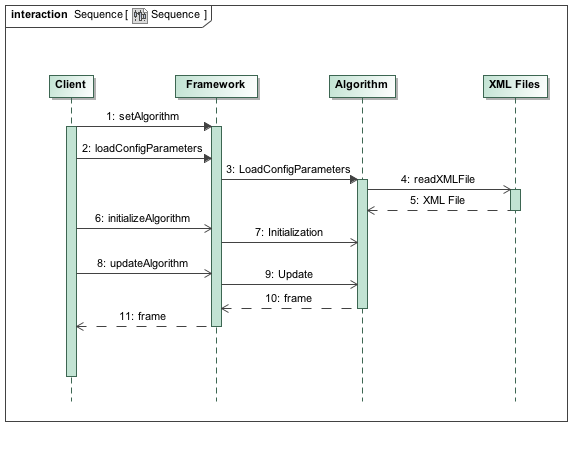
\includegraphics[scale=0.5]{img/Sequence}
\caption[Diagrama de secuencia]{Diagrama de secuencia de ejecución de un algoritmo}
\label{fig:uml_sequence}
\end{figure}


El diagrama de secuencia de la figura \ref{fig:uml_sequence} muestra un ejemplo de los mensajes que son intercambiados entre un cliente, el \textit{framework} y un algoritmo. El cliente inicia enviando un mensaje al objeto \textit{framework} para indicar el tipo de algoritmo a utilizar. Luego, el cliente pide configurar, esto activa un mensaje desde el \textit{framework} hacia el algoritmo señalado, en el paso anterior. En la parte de inicialización se configura el algoritmo con parámetros por defecto. Finalmente, el cliente envía un mensaje de ``update'' que significa obtener una nueva mascara de foreground.


\subsubsection{Herramienta de evaluación}
Este módulo es una clase que define en cada una de  programa principal, que 
\chapter{Experimentación}


\chapter{Conclusiones}\label{chap:conclusiones}

%Este trabajo de tesis se propuso como objetivo principal implementar un sistema de software, que permitiese en una primera parte la incorporación de algoritmos de sustracción de imágenes de fondo, empleados en el campo de investigación de visión por computador. Y en una segunda parte el desarrollo de una herramienta de evaluación de desempeño, independiente de los algoritmos incorporados en este sistema, que incluyera un conjunto de métricas empleadas comúnmente en visión por computador (u otras disciplinas de maquina de aprendizaje computacional, reconocimiento de patrones, sistemas de recuperación de información, etc) y funcionase como un sistema de evaluación independiente, con la finalidad de evaluar sólo mascaras de imágenes resultantes sin necesidad de conocer la base de funcionamiento de algún algoritmo en evaluación. El proyectoTodo este 

%para finalmente terminar nuevamente vinculados en el resultado final de este proyecto de tesis

Este trabajo de tesis fue desarrollado en base a tres dimensiones. En la primera parte se propone el objetivo principal de implementar un sistema de software, que permitiese la incorporación de algoritmos de sustracción de imágenes de fondo, empleados en el campo de investigación de visión por computador. En una segunda parte se proyecta el desarrollo de una herramienta de evaluación de desempeño, independiente de los algoritmos incorporados en este sistema, que incluyera un conjunto de métricas utilizadas comúnmente en visión por computador (u otras disciplinas de maquina de aprendizaje computacional, reconocimiento de patrones, sistemas de recuperación de información, etc) y además funcionase como un sistema de evaluación autónomo, con la finalidad de evaluar sólo mascaras de imágenes resultantes sin necesidad de conocer la lógica de funcionamiento del algoritmo en evaluación. Y un último aspecto se relaciona con el conjunto de datos MuHAVI, que actúa como el componente de evaluación del desarrollo de este proyecto de tesis, en base a este conjunto de datos surgen desafíos que se fueron superando durante las distintas etapas de trabajo. 

Una de las salidas de este proyecto corresponde al sistema de software, que incorpora un grupo de algoritmos basados principalmente en mixtura de componentes Gaussiano, orientados a realizar sustracción de imágenes de fondo, procedimiento también denominado por sus nombres en ingles, \textit{Background Subtraction} o \textit{Foreground and Background separation}. La implementación del software utiliza como sustento el conjunto de biblioteca de clases C++, disponibles en la plataforma abierta de visión por computador \textit{OpenCV} y desarrollado en una plataforma \textit{Linux} de 32 bits. El sistema final corresponde a un conjunto de bibliotecas C++, archivos xml de configuración y un grupo de programas de computación que permiten la ejecución y utilización de estos algoritmos de visión por computador en cualquier secuencia de video disponible.  Este software tiene la flexibilidad de incorporar nuevos algoritmos, y requiere para esto las clases y métodos empaquetadas en una biblioteca tipo \textit{Linux}. Sin embargo, este último requerimiento crea una restricción importante, y deja fuera por incompatibilidad de sistema operativos, una buena parte de antiguos y nuevos prototipos que la comunidad de investigación en este campo está desarrollando.

El segundo producto del proyecto se manifiesta como respuesta a la inquietud de una búsqueda de evaluación de los algoritmos incorporados en el sistema anterior. Interesaba saber de manera imparcial el rendimiento de los algoritmos utilizados en un conjunto de datos como MuHAVI. Se hace una investigación y se evidencia que existen bastantes métricas de evaluación de desempeño, y la mayoría de ellas basadas en discrepancia, es decir, comparación de una imagen resultado (mascara) con su referencia. En este proyecto se implementa una herramienta que incluye varias de estas métricas, cada una de ellas destaca en forma individual alguna característica de un algoritmo, pero en su conjunto entregan una visión más completa de desempeño. El software es un programa ejecutable que admite dos entradas, las mascaras binarias (imágenes de siluetas) y las referencias (\textit{ground-truth}), el resultado es un archivo de texto con un resumen por imagen de las mediciones realizadas por el programa. Las métricas integradas más importantes, se fundamentan en el resultado de clasificación a nivel de pixel. El programa identifica si un pixel ha sido bien seleccionado y a partir de esa comparación puede determinar el nivel de clasificación de un algoritmo. Identifica el nivel de `\textit{especificidad}' y `\textit{sensitividad}', es decir, realiza una medición de la proporción de positivos y negativos correctamente clasificados. Estas dos mediciones permiten generar un número distinto de métricas orientadas a responder diversas preguntas en la evaluación de desempeño. En el transcurso de la experimentación se logra determinar que el coeficiente de correlación \textit{MCC} y \textit{F-Measure}, en este proyecto, se pueden considerar mediciones de desempeño equivalentes. Lo mismo sucede con las métricas de \textit{PSNR} y \textit{MSSIM} las dos producen similares resultados, por lo que no se requiere la utilización de ambas. Una de las mediciones más relevantes encontradas durante este trabajo, es la métrica \textit{D-Score}, la cual entrega una medición que descarta los falsos positivo lejanos y pondera mayormente los pixeles falsos positivos cercanos a la forma del objeto (siluetas en este  proyecto) que se intenta reconocer, de esta manera, se corrobora que esta métrica entrega una buena indicación, de la factibilidad de reconocer la forma de la silueta en procesos posteriores. El mayor inconveniente de esta métrica es el extensivo procesamiento computacional, realiza extensos cálculos de distancia que condiciona su uso a la potencia del equipamiento usado. De todas manera esta restricción computacional en un futuro cercano no será inconveniente, por el vertiginoso avance en potencia de los equipos de computación.

Una tercera parte de este proyecto, es el análisis de los resultados de la experimentación. Todas las conclusiones de desempeño de los algoritmos, se basan en los análisis de mediciones globales promedios obtenidas durante la experimentación. Una medición es el promedio general de resultados parciales de ejecuciones realizadas sobre cada secuencia del conjunto de datos MuHAVI. El promedio de mediciones por algoritmo es un indicador global, que oculta el desempeño particular de los algoritmos evaluados sobre alguna secuencia específica. MuHAVI expone desafíos adicionales, fuera del problema básico de reconocer una acción humana, que puede interesar observar en la evaluación final y se ocultan en las mediciones globales resultantes. El tipo iluminación usado en la construcción de este conjunto de datos genera problemas que pueden resultar difíciles de resolver por los algoritmos e incide en el deterioro de su desempeño final; estos son figuras fantasmas (sombras de las actores proyectadas en el escenario por más tiempo de lo necesario), cambios pequeños en la iluminación global que puede confundir al algoritmo e invertir el reconocimiento de una figura del fondo (o viceversa), y las sombras de los actores proyectadas en el escenario que se confunden como una extensión de la figura humana. Sin embargo, el promedio general de las mediciones en su conjunto construye un buen indicador de desempeño de los algoritmos. La etapa de experimentación por ejemplo ha determinado, contrastando curvas de operaciones y comparando las mediciones de las métricas desempeño, que el algoritmo \textit{SAGMM} presenta  rendimiento mejor con respecto a los otros algoritmos, y esto se confirma visualmente al observar algunas imágenes de resultados tomadas al azar, que ratifican la calidad de la silueta con respecto a los algoritmo similares.

Con respecto al desempeño individual de los algoritmos escogidos. Se ha demostrado por ejemplo que el algoritmo de Zezhi Chen \cite{chen_vehicle_2012} denominado \textit{SAGMM} es una mejora del algoritmo de \textit{Zivkovic y Heijden} \cite{zivkovic_efficient_2006} denominado \textit{MOG2} (\textit{Mixture Of Gaussians}). \textit{SAGMM} agrega esencialmente dos nuevos componentes al algoritmo original. Incorpora, en la etapa previa de procesamiento, un filtro de procesamiento temporal (cadena continua de cuadros dentro de una secuencia) y espacial (filtro gaussiano entre pixeles de un vecindario) que favorece la estabilidad a nivel de imagen y posibilita mejor discriminación de componentes gaussianos durante el procesamiento del algoritmo. Asimismo incluye un factor de iluminación global con el propósito de compensar cambios bruscos de luminosidad. Estos dos nuevos elementos se evidencian en el mejor desempeño de éste sobre \textit{MOG2}. La implementación de este algoritmo, junto con MOG2,  forma la base del sistema desarrollado para este proyecto. A pesar, que los algoritmos UCV \textit{Staircase} y \textit{Linear} presentan un desempeño desmejorado con respecto a los otros basados en mixtura de componentes Gaussianas, estos algoritmos están orientados a ser incorporados en sistemas embebidos basados en micro-controladores, en consecuencia abordan restricciones y complejidades que constituyen las fortalezas y ventajas de \textit{UCV}, que los otros algoritmos no consideran dentro de sus diseños. Esto último revela una carencia de este trabajo, y es dejar fuera las métricas de evaluación de los tiempos de ejecución, o la medición de la cantidad de recursos computacionales (el uso de memoria o carga de CPU) requeridos por un algoritmo. Estas mediciones agregarían una nueva dimensión a la evaluación global y van en el camino de destacar particularidades que pueden tener los algoritmos y no se reflejan en el contexto global. 

MuHAVI por su parte es un conjunto de datos que proporciona con muchas vistas (disposición de cámaras en diferentes ángulos) de la misma acción (o del conjunto de acciones), eso conlleva resultados con diferentes varianzas de las mediciones globales. La última parte de la experimentación intenta identificar estas varianzas en el resultado global de la curva de operaciones, al obtener los intervalos de confianza del resultado promedio, y generar un rango (o banda) de valores con una probabilidad del 95\% donde se localiza el resultado. Pero se necesita un análisis estadístico más extenso de los resultados, el estudio de los intervalos de confianza sólo considera 20 muestras globales generales por algoritmo (promedio de 5 secuencias, con 2 actores y 2 cámaras) y considera una distribución de muestreo normal de la media de las muestras, para hacer inferencia estadística de la curva de operaciones. Este mismo estudio se podría hacer considerando por ejemplo una distribución binomial por la naturaleza binaria de las muestras (pixel de una imagen en dos estados) o bien una distribución t (\textit{Student}) por el tamaño pequeño de las muestras. Igualmente, se asumió una distribución normal subyacente al estimar la media estadística del resultado de una secuencia como un indicador global (promedio de la tasa de verdadero y falsos positivos). El conjunto de valores que resultan del procesamiento de una secuencia (por algoritmo) constituye un cluster de valores que no necesariamente se pueden estimar como una distribución normal (o binormal con ambos valores), esto por consiguiente deja abierta la inquietud de considerar el promedio general como un buen indicador global de rendimiento. De esta forma se podría buscar otra estadística que mejor identifique el respuesta de un algoritmo, por ejemplo usar la mediana en vez del promedio. Un trabajo futuro debiera intentar estimar la distribución subyacente de los resultados de una secuencia; estimar los sesgo de la distribución, modelar como una distribución binomial, o usar un modelo no-paramétrico para estimar las distribuciones del resultado de procesamiento de las secuencias. Por otra parte, no queda claro donde surge la variabilidad de los resultados, se puede relacionar esta variabilidad con la respuesta de los algoritmos a los cambios sutiles de iluminación en MuHAVI, afecta el color de la ropa de los actores (ropa oscura en un escenario con poca iluminación) en el resultado global.

Finalmente como trabajo futuro, queda pendiente incorporar un nuevo módulo en el sistema de software que implemente algún algoritmo de reconocimiento de acciones. Con el propósito de corroborar los resultados obtenidos en este trabajo de tesis, verificar que los algoritmos evaluados con buen desempeño entregan una buena base para realizar reconocimiento de acciones. Esto abre nuevas preguntas, las métricas para evaluar los algoritmos estudiados sirven igualmente para evaluar los algoritmos de detección de acciones, se necesitaría un tipo diferente de métricas, el concepto de discrepancia como método de evaluación sigue siendo válido en detección de acciones. En la misma línea, pero por el lado de la implementación de software, es necesario, que todos los algoritmos que se implementen a futuro usen alguna técnica de paralelismo, como cluster con tarjetas GPU, esto reduciría sin duda enormemente los tiempos de experimentación, pero introduce los desafíos técnicos de implementar estos algoritmos en kernels GPU para la ejecución.


%- Quedan fuera los tiempos de ejecución, incorporar GPU
%- Box, zona de interes
%
%
%
%
%De esta forma se podría encontrar una estadística que mejor identifique la respuesta de una algoritmo, por ejemplo usar mediana en vez del promedio, o reconocer el sesgo de la distribución estadística de respuesta. 
%
%. No queda claro en este trabajo de donde surge la variabilidad de las respuestas, o porque las respuestas en las curvas de operaciones se alejan de la curva promedio. SE puede relacionar el factor de iluminación de MuHAVI con la variabilidad que se encuentra en el resultado de las distintas secuencias. Afecta el color de la ropa de los actores en los resultados  el valque el algoritmo  el problema de las diferentes varianzas en el  
%
%
%
%   distribución o  
%
%deja la inquietud queda abierto  y en consecuencia tampoco se podría considerar la estadística . Una alternativa de este trabajo, por ejemplo, puede consistir en utilizar la mediana en vez de la media, un estudio más detallado resultado de cadaLa salida de cada secuencia (por algoritmo) es en si mismo de cada secuencia es en si mismo un cluster . , pero  nivel de secuencia se toma como indicador global la estadística de la media Por otra parte, el estudio a nivel de secuencia, se considera la media estadística como un indicador global del resultado estadístico (con m) un número el número estadístico que se obtiene como indicador global es la media  parte la estadística que se obtien
%
%Las curvas ROC es una herramienta muy utilizada en el campo del diagnóstico médico, las cuales se han llevado para el análisis de clasificación binaria y estas mismas herramientas se sus desde ese campo se han desarrollo los pero  Se requiere, por ejemplo, identificar el tipo de distribución estadística que está parte requiere más profundización. Por ejemplo, se podría identificar el tipo de distribución estadística que tienen por secuencia los resultados de verdadero y falsos positivos. 
%La continuación de este trabajo 
%
%fue el tiempo de toma una ejecución completa de una secuencia, o la cantidad de recursos computacionales que se necesitan para utilizar estos algoritmos. En estos dos aspectos, \textit{UCV} tiene una ventaja competitiva.   en este ambiente Se incluye también otros dos algoritmos basados en mistura de Gaussianas, pero orientados a sistemas embebidos tipo micro-controladores. Finalmente el desarrollo de esta etapa microncontroladores También incluye dos algoritmos que Este algoritmo se incorpora en el sistema base de este proyecto, la base del sistema implementado. 
%
%Sin embargo, a pesar del comentario anterior, es importante reconocer que el promedio global nos da un buen indicador del desempeño de los algoritmos. En la etapa de experimentación se ha determinado que el algoritmo \textit{SAGMM} ha tenido un bueno desempeño, las cifras globales de los resultados indican que este algoritmo tiene un rendimiento mejor que los demas evaluados. Esto se comprueba 
%
%
%  de los n el reconocimiento de colores y generar zonas de siluetas los colores de iluminación que provoca confunden lprovocan en ciertas partes del escenario  la secuencia tiempo después que el actor  El problema de la iluminación  resulta interesante evaluar el comportamiento de los algoritmos. Por ejemplo, un par de problemas en varias de sus secuencias    
%
%
%
%  parciales viene  se basan sobre análisis se basan sobre realizados corresponden a mediciones globales de desempeño, es decir, por cada una de las ejecuciones realizadas sobre las secuencias del conjunto de datos MuHAVI, se obtuvo un promedio de mediciones definidas en la herramienta de software, posteriormente, una vez que se fueron realizadas todas las ejecuciones del algoritmo sobre las secuencias, se obtuvo un promedio general con los promedios de todas las secuencias. 
%Este promedio de métricas de desempeño por algoritmo es en un indicador global, que puede ocultar muchos de los desafíos particulares que tienen las secuencias y no dice mucho como el algoritmo que está en evaluación lo resuelve. Por ejemplo varias secuencias de MuHAVI presentan problemas que se denominan fantasmas, es decir queda proyectada la sombra del actor más después que ésta ha dejado el escenario. Un algoritmo que no maneja bien este problema reporta un aumento en su cantidad de falsos positivos en esa secuencia, pero será atenuada por el resultado de las otras secuencias. Lo mismo sucede con los cambios bruscos de iluminación, es muy difícil, reconocer en términos globales el comportamiento de una algoritmo frente estos problemas mencionados, y que MuHAVI los contiene como una característica propia. 
%
%
%
%

%  , pero  particularidades de las secuencias y el la herramienta de software una de las métricas, para finalmente promediar esos resultados promedios por secuencia y así obtener un promedio general hizo un promedio de las métricas se seleccionó un algoritmo del sistema  un algoritmo 
%
% para que posteriormente sea segmen. Este ha resultado ser un buen indicador mediciones de de de la clasificación se fundamentaLas métricas integradas consisten en mediciones de 
%
%El software desarrollado permite agregar  la biblioteca de clases de vision por computador C++  La primera parte, corresponde a una de las salidas de este proyecto. Este consiste de una sistema de software que se compone de una plataforma base la producto que este proyecto entrega al sistema implementado  que corresponde al sistema implementado, cEl sistema implementado consiste de un grupo de algoritmos basados en una mixtura de componentes gaussianos. , la base del programa  
%La implementación (migración desde Matlab) del algoritmo \textit{SAGMM} \cite{chen_vehicle_2012}, es parte de los objetivos específicos planteados al inicio. Se utiliza para este propósito el conjunto de clases y bibliotecas que dispone la plataforma de visión por computador \textit{OpenCV}. Gran parte de esta primera parte se deriva en entender el funcionamiento de los algoritmos basado en mixtura de componentes Gaussianos, y principalmente el trabajo propuesto por \textit{Zivkovic y Heijden} \cite{zivkovic_efficient_2006}. Esto debido que el algoritmo Zezhi Chen \cite{chen_vehicle_2012} denominado \textit{SAGMM}, propone dos mejoras del algoritmo de estos últimos autores mencionados y es denominado \textit{MOG2} (\textit{Mixture Of Gaussians}). Esencialmente el algoritmo \textit{SAGMM}  incorpora en una etapa previa un filtro de procesamiento temporal (cadena continua de cuadros dentro de una secuencia) y espacial (filtro gaussiano entre pixeles de un vecindario) que favorece la estabilidad de nivel de imagen y posibilita mejor discriminación de componentes gaussianos durante el procesamiento del algoritmo, y como el desarrollo de esta algoritmo surge en el campo de la vigilancia, agrega un factor iluminación global que compensa bruscos cambios de luminosidad. La implementación de este algoritmo, junto con MOG2,  forma la base del sistema desarrollado para este proyecto. Se incluye también otros dos algoritmos basados en mistura de Gaussianas, pero orientados a sistemas embebidos tipo micro-controladores. Finalmente el desarrollo de esta etapa microncontroladores También incluye dos algoritmos que Este algoritmo se incorpora en el sistema base de este proyecto, la base del sistema implementado 
%
%agrega un filtro de iluminaci. Una segunda procesamiento gaussiano)ees un filtro temporal y espacial que mejora la estabilidad de una imagen a nivel de pixel y mejora  de las secuencias de entrada el algoritmo se basa en este último   propuesto por  El algoritmo , de se utiliza para este efecto la plataforma de visión por computador \textit{OpenCV}, la cual ofrece muchas bilbioteca de clases en C++ utilizando par 
%Se requiere de un conjunto de datos con desafíos que emulen los aspectos de la vida diaria y real importantes. Se requiere de un conjunto de datos con desafíos reales para evaluar y mejorar los algoritmos desarrollar, para    Y una último aspecto que incTodo esto El proyectoTodo este 
%Desde el mundo de los algoritmos surgen ideas bla bla bla 
%
%Ambos sistemas de software (base de algoritmos, y herramienta de evaluacion de desempeño) fueron implementados y verificados con diferentes algoritmos. El primer tiempo del proyecto se inicio con la implementación del algoritmo SAGMM \cite{chen_vehicle_2012}  se inicio con el desarrollo del algoritmo  , y el tiempo de desarrollo necesito más tiempo del proyectado.    independientes fueron implementados, y tuvieron un tiempo de desarrollo fueron totalmente implementados 
%
%El desarrollo del sistema de software utiliza sistema de software está 
%La etapa de desarrollo requiere 
%
%Este proyecto nace de la necesidad de consolidar distintas métricas de evaluación que destacan alguna característica específica de los algoritmos, pero en la comunidad de investigación por computador no se utiliza un conjunto completo que evalúen diferentes dimensiones y entreguen una idea global de desempeño.
%
%que den idea global de desempeño el mundo existen diferentes métricas que  y se ocupa MuHAVI como conjunto de datos independientes  de manera de evaluar sólo las mascaras de imágenes resultantes sin necesidad de recurrir al algoritmo siendo evaluando que evaluase la salida resultado sin necesidad de requerir el algoritmo para realizar su experimentación. 
%
%
% evaluación. Sólo se requiere del salida . Se trata de  de un algoritmo para evaluar el resultado. l algoritmo que permitiese un sistema de evaluación independiente de  sistemas de recuperación de información, reconocimiento de patrones, y permitiese  . Pde estos algoritmos , como con un modulo que incluyera, o permitiese la fácil incorporación, de un conjunto de algoritmos muy empelados en el campo de la visión por computador, como los software de sustracción de imagenes de fondo y ademas otro módulo que implementara un conjunto de métricas de evaluación de desempeño de estos algoritmos. 
%
%
%realizara la eval agregar nuevos software en el futuro, un conjunto de algoritmos de muy utilizados en el campo de investigación de visión por computador en el futuro alque incorporara un modulo con  una bloque dos bloques principales. Una parte que permita  implementar un
%
%This dissertation addressed a framework for object detection, tracking and vehicle classification in an urban environment. A generalized active contour model for multi-channel and multi-phase colour image segmentation and an adaptive object-tracking algorithm have been proposed. By using level set methods, the mean shift tracking algorithm, a Chamfer distance transform (NCDT kernel) and sorted CSMs, objects can be detected and tracked. Their boundaries are not necessarily defined by a gradient or by very smooth boundaries, and hence classical active contour models are not applicable. The position of the initial curve can be anywhere in the image, and it does not necessarily surround the object to be detected. However, if the initial estimate is far from the true contour, it takes a long time to converge to the optimal solution. Several experiments have demonstrated the ability of the model to detect and track an object in movie sequences. Comparing the new method with the CVV method, the comparisons also show that the method proposed in the thesis is more accurate and robust in terms of image segmentation in the presence of symmetric and asymmetric noise.


%  Appendix
%\appendix
%\include{src/appendix}



%  Bibliography
\bibliographystyle{plain}
%\bibliographystyle{chicago}
%\bibliographystyle{unsrtnat}  % Use the "unsrtnat" BibTeX style for formatting the Bibliography
%\bibliographystyle{ieeetr}
\bibliography{biblio/bibliografia}

\end{document}




